%%中山大学物理学院-基础物理实验-论文格式报告模板1.1
%%完成整理日期:2020/2/18
%%更新时间:2020/8/25
%%中山大学物理学院18级 王佛泓
%%文本编辑器:Sublime Text
%%平台:win10, Texlive 2019

%---------------------导言区---------------------------%
\documentclass[10pt,a4paper,twocolumn,twoside,UTF8]{ctexart}
	%10pt:正文字体为10pt,可以缺省;各层级字体大小会根据正文字体自动调整
	%a4paper:纸张大小a4;
	%twocolumn:双栏排版;
	%twoside:排版上分奇偶页,一般也就是有双面打印的需求;
	%UTF8:中文要求
\usepackage{geometry}%用于设置上下左右页边距
	%左右边距一样: 不考虑装订和翻页的需要.实验室网站上的示例论文格式报告就是这样。
	\geometry{left=2cm,right=2cm,top=2.5cm,bottom=4cm}
	%实际上,一般需要考虑到双面打印、装订和翻页的需要,需要区分奇偶页。奇偶页的页边距需要分开设置。奇数页左边距较宽,偶数页左边距较窄。
\usepackage{xeCJK,amsmath,paralist,enumerate,booktabs,multirow,graphicx,float,subfig,setspace,listings}
	%xeCJK:中文字体(如楷体,作者和机构需要用到)的设置
	%amsmath:数学公式
	%paralist,enumerate:自定义项目符号
	%booktabs:三线图,论文常用的表格风格
	%multirow:复杂表格
	%graphicx,float: 插入图片
	%subfig:并排排版图片以及强制图表显示在“这里”[H]
	%setspace:设置行间距等功能
	\setlength{\parindent}{2em}%正文首行缩进两个汉字
	%listings:用于排版各种代码;比如matlab的代码
	\lstset{language=Matlab}%matlab代码
	%代码环境的使用可以参考完整实验报告模板

\setCJKmainfont{HGSS1_CNKI}%中文字体:华光书宋一

\usepackage{titlesec}
	%改变section、subsection里面字体的样式。中文黑体,英文TNR。
	\newfontfamily\sectionef{Times New Roman}
	\setCJKfamilyfont{FZHeiTi}{SimHei}
	\newcommand{\sectioncf}{\CJKfamily{FZHeiTi}}
	\titleformat*{\section}{\large\bfseries\sectioncf\sectionef}
	\titleformat*{\subsection}{\normalsize\bfseries\sectioncf\sectionef}
	\titleformat*{\subsubsection}{\normalsize\kaishu}

\usepackage{fancyhdr}
	%fancyhdr:一个很强大的宏包,用于自定义设计页面风格并命名以供调用。

\newcommand{\newtitle}{数字全息记录和光学实时再现实验}


%%begin----------设置首页和正文不同的页眉页脚----------------%%

\usepackage{ifthen}%这个宏包提供逻辑判断命令
\newboolean{first}%引入布尔变量
\setboolean{first}{true}%将布尔变量设置为true
\pagestyle{fancy}

	%%% Step1 定义正文的页面风格
	%E表示偶数页,O表示奇数页;R、L、C代表文字居右、居左、居中排版
	%页码:保证在外侧, 奇数页分布在右边,偶数页分布在左边
	%页眉中间的内容也因奇偶页而不同
	%实验名称根据实际情况修改
	\fancypagestyle{maincontent}{
		\fancyhf{}  %清空页眉页脚设置
		\fancyhead[EL, OR]{\thepage}
		\fancyhead[EC]{\newtitle}
		\fancyhead[OC]{\newtitle}
		\renewcommand\headrulewidth{0pt}
	}

	%%% Step2 定义首页的页面风格
	%页眉中间的双行文字,大小和字间距需要微调
	%左右的内容是年月,可以自己修改寻找自动获取的方法
	\usepackage{datetime}
		%\shortmonthname可以获取英文月份缩写
	\fancypagestyle{firstpage}{
		\setboolean{first}{false}%firstpage出现,则将first重置为false
		\fancyhf{}  %清空页眉页脚设置
		\fancyhead[L]{\the\year 年\the\month 月}
		\fancyhead[R]{\shortmonthname[\the\month], \the\year}
		\fancyhead[C]{\normalsize\kaishu 武汉大学物理科学与技术学院\\物理实验报告
		          }
	}

	%%% Step3 页眉线的设置:用布尔变量区分首页和正文
	\newcommand{\makefirstpageheadrule}{%定义首页页眉线-双线绘制命令
		\makebox[0pt][l]{\rule[0.55\baselineskip]{\headwidth}{0.2pt}}%上0.5pt,下0.2pt
		\rule[0.7\baselineskip]{\headwidth}{0.5pt}
	}

	\newcommand{\makeheadrule}{%定义正文页页眉线绘制命令,单线
		\rule[0.7\baselineskip]{\headwidth}{0.75pt}
	}

	%根据布尔变量first为true或false分别执行不同的页眉线绘制命令
	\renewcommand{\headrule}{%重定义headrule命令
		\ifthenelse{\boolean{first}}{\makeheadrule}
		{\makefirstpageheadrule}
	}



%%end--------------设置首页和正文不同的页眉页脚-----------%%



%%begin-----------------参考文献-----------------------%%

\usepackage[citecolor=black]{hyperref}%超链接
% % \usepackage[hyperref=true,backref=true]{biblatex}
% 	%hyperref=true和backref=true表示为各个参考文献的引用处、及定理、定义、例子等的引用处都添加上超链接;
% 	%backend=biber:后端处理的程序为biber.exe
% 	%bibstyle:参考文献风格;每个期刊、组织要求不同
% 		%gb7714-2015是目前国内期刊通用的风格,称为gb标准风格
% 	%citestyle:引用风格;每个期刊、组织要求不同
% 	%sorting=none:按照参考文献在论文中出现的先后顺序排序。
% 	%**编译:biblatex与biber命令配合使用。xelatex-biber-xelatex-xelatex
\hypersetup{ %设置链接的颜色为不可见
	colorlinks=true,
	linkcolor=black
	}
%%end-------------------参考文献-----------------------%%




%%%%%%%%%%%%%%%%%%%%%%%%%%%%%%%%%%%%%%%%%%%%%%%%%%%%%%%%%%
%%%%%%%%%%%%%%%%%%%%%%%%%正文开始%%%%%%%%%%%%%%%%%%%%%%%%%%
%%%%%%%%%%%%%%%%%%%%%%%%%%%%%%%%%%%%%%%%%%%%%%%%%%%%%%%%%%

\begin{document}

%%begin-------------------中文摘要-----------------------%%
\title{\heiti \newtitle}
\author{\zihao{3}\kaishu 周澳\quad 2018302020200}
\date{}%不显示日期

\twocolumn[
	%twocolumn: 双栏article下的单栏摘要
	\begin{@twocolumnfalse}
	\maketitle  %标题和作者
  	\renewcommand{\abstractname} {} %不显示摘要名字
	\begin{abstract}
	\vspace{-3em}
	%vspace:调整垂直空白,可以自己调整;缩小abstract和center(以及maketitle)的间距
	%\noindent %备用:摘要无缩进
	{\heiti 摘\ 要:}
	{\small 数字全息与传统光学全息相比有更大的灵活性,其显著的好处在于可以不使用全息干板作为记录介质,还有可消除像差、噪声及记录过程中底片非线性等因素的影响的优势。本文介绍了数字全息记录和再现的原理,并分别进行了光学方法和计算模拟方法的的全息图的记录和再现实验。}
	\par%空的新行的高度。
	{\heiti 关键词:}
	全息术 \quad 数字全息记录 \quad 光学全息再现 \quad 计算模拟全息
	\vspace{0.5em}
	\end{abstract}
	\begin{center}%
	    {\large\bfseries Digital Recording and Real-time Optical Reconstruction of Hologram\par}%
		\vskip 0.8em%
		{Ao Zhou\quad 2018302020200}
	\end{center}
	\begin{abstract}
	\vspace{-3em}  %缩小abstract和center(以及maketitle)的间距
	{\bf Abstract:}
		{\small Digital holography has much more flexibility compared with traditional optical holography, one of which is that digital holography does not need holographic plate as recording material, and it has advantages in elimination of aberrations and nonlinearity ect. This article introduces principles of digital holographic recording and reconstruction, and conducted experienments on holographic recording and reconstruction by both optical and computer simulation methods.}
	\par%空的新行的高度。
	\textbf{Key words}:Holography, Digital holographic recording, Optical holographic reconstruction, Computer simulating holography
	\vspace{2em}
	\end{abstract}
	\end{@twocolumnfalse}
]
\setlength{\parskip}{0.5em} %设置段落间距
%%end-------------------中文摘要-----------------------%%

\thispagestyle{firstpage}%首页页面风格:firstpage
\pagestyle{maincontent}%第二页之后的页面风格:maincontent

%%begin----------------层级结构------------------------%%

%重点1:知道每一个层级的样式和怎么和后面的正文接上
%重点2:掌握各种换段的方法
%重点3:自定义的项目符号(宏包enumerate的用法)

	\section{引言}
	全息干涉测量是一种非常有用的无损检测技术,然而,用传统全息干板记录全息图时必须做显影等湿处理,在实际应用中有许多不便。 1967 年由Goodman等人便开始用 CCD 摄像机记录干涉图。 1971 年, Huang 在介绍计算机在光波场分析中的进展时,首次提出数字全息的概念,进入 21 世纪数字全息已经成为一个十分活跃的研究领域。

	\section{实验原理}
	全息技术是基于光的干涉原理,将物体发射光波波前以干涉的形式记录光波的相位和振幅信息,利用光的衍射理论再现所记录物光波的波前,从而获得物体振幅和相位信息,此类技术在光学检测和成像方面有着广泛的应用。传统光学全	息实验是通过银盐、重铬盐材料或光致聚合物等记录全息图 ,拍摄过程对环境要求较高,冲洗过程繁琐 ,重复性差。
	
	本实验在传统全息术基础上,开发了数字全息、计算模拟全息和光学实时再现等全息技术。数字全息技术自1967年顾德门提出,其基本原理是用高分辨率摄像机代替干板或者 光致聚合物记录全息图,然后由计算机模拟光场对全息图进	行数字再现。计算模拟全息是利用计算机模拟物光和参考光通过计算获得模拟全	息图,通过计算机模拟光场实现数字再现。光学实现再现是将模拟全息图或数字	全息图加载到空间光调制器,同时用参考光照射,在空间光调制器后面即可用白屏或 CCD 接收再现图像。
	
	数字全息记录和再现的基本理论与普通全息是相同的,其区别在于数字全息采用数字摄像机代替干板存储全息图,通过计算机软件模拟记录光场实现图像衍射再现,简化了再现过程,实现了全息图实时记录与存储,展现了全息的数字化过程。

	\subsection{数字全息的全息图记录}
	物光波的信息包括光波的振幅和相位,然而现有的记录介质均只能记录光强,因此,必须把相位信息转换为强度信息才能记录下物光的所有信息。全息术就是利用干涉法将空间相位调制转化为空间强度调制从而记录下物光波全部信息的方法。

	图\ref{yuanli}为数字全息记录和再现的坐标系统变换示意图。物体位于物平面$x_0y_0$面上,与全息平面$xy$面相距$d_0$ ,即全息图的记录距离。摄像机位于$xy$面上,记录物光和参考光在全息平面上的干涉光强分布。$x_Iy_I$面是数值再现的成像平面,与全息平面相距$d$,也称为再现距离。
	\begin{figure}[H]
		\centering
		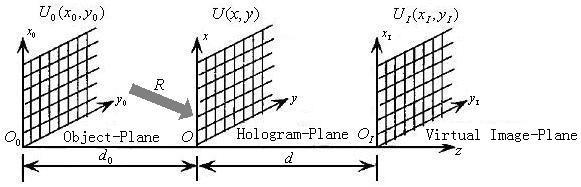
\includegraphics[width=0.4\textwidth]{img//yuanli.jpg}
		\caption{数字全息图记录和再现的坐标系统变换示意图}
		\label{yuanli}
	\end{figure}

	设位于$x_0y_0$平面的物光场分布为$U_0(x_0,y_0)$,传播到全息平面$xy$面记为
	\begin{equation}
		O(x,y)=A_0(x,y)\exp \{j\phi_o(x,y)\}
		\label{Oxy}
	\end{equation}
	其中$A_0(x,y)$和$\phi_o(x,y)$分别为物光波的振幅和相位分布。将到达全息平面上的参考光波记为
	\begin{equation}
		R(X,y)=A_r(x,y)\exp \{j\phi_r(x,y)\}
		\label{Rxy}
	\end{equation}
	其中$A_r(x,y)$和$\phi_r(x,y)$分别为参考光的振幅和相位分布。则$xy$面上的全息图光强分布为
	\begin{equation}
		I_H(x,y)=|U(x,y)|^2=|O(x,y)+R(x,y)|^2
	\end{equation}
	将式(\ref{Oxy})和(\ref{Rxy})代入上式可得
	\begin{equation}
		\begin{aligned}
		&I_H(x,y)\\ &=|A_o(x,y)|^2+|A_r(x,y)|^2+\\ &O(x,y)R^*(x,y)+O^*(x,y)R(X,y)\\ &=|A_o(x,y)|^2+|A_r(x,y)|^2+\\ &2A_o(x,y)A_r(x,y)cos[\phi_o(x,y)-\phi_r(x,y)]
		\end{aligned}
		\label{holoeq}
	\end{equation}
	式(\ref{holoeq})的前两项分别是物光和参考光的强度分布,仅与振幅有关,与相位没有关系。第三项是干涉项,包含了物光波的振幅和相位信息。参考光波作为载波,其振幅和相位都受到物光波的调制,干涉条纹则是参考光波的振幅和相位受到物光波调制的结果。

	由于数字全息是使用CCD代替全息干板记录全息图,因此想获得高质量的数字全息图,并完好重现物光光波,必须保证全息图表面上的光波的空间频率与记录介质的空间频率之间满足奈奎斯采样定理,即记录介质的空间频率必须是全息图表面上光波的空间频率的两倍以上。。由于现有摄像机分辨率较低,因此只有尽可能减小参考光和物光夹角才能保证携带物体信息的物光中的振幅和相位被全息图完整的记录下来。摄像机的像素尺寸一般在5-10微米范围内,故参考光和物光夹角最大值在2-4度范围内。

	\subsection{计算模拟全息的记录}
		\subsubsection{物面和全息图面的抽样及计算}
		数字计算机通常只能对离散的数字信号进行处理,并以离散的形式输出。因此,制作计算全息图的第一步是对物波函数进行抽样。设待记录的物波函数为
		\begin{equation}
			f(X,y)=a(x,y)\exp\{i\phi(x,y)\}
		\end{equation}
		其傅里叶变换(空间频谱)为
		\begin{equation}
			F(u,v)=A(u,v)\exp\{i\psi(u,v)\}
		\end{equation}
		对于傅里叶变换全息图,全息图上记录的是物波的空间频谱$F(u,v)$,因此必须对物波函数进行离散傅里叶变换。离散傅里叶变换的公式如下:
		\begin{equation}
			F(j,k)=\sum\sum  f(m,n)\exp\{-i2\pi(\frac{jm}{M}+\frac{kn}{N})\}
		\end{equation}
		通常使用快速傅里叶变换算法(FFT),计算结果一般为复数:
		\begin{equation}
			f(m,n)->F(j,k)=F_r(j,k)+iF_i(j,k)
		\end{equation}
		其振幅和相位可分别表示为
		\begin{equation}
			\begin{aligned}
			&A(j,k)=\sqrt{F_r^2(j,k)+F_i^2(j,k)},\\ &\psi(j,k)=tan^-1\frac{F_i(j,k)}{F_r(j,k)}
			\end{aligned}
		\end{equation}

		\subsubsection{编码及绘制全息图}
		编码的目的就是将计算出的全息图面上的复振幅函数转化成实值函数(全息图透过率函数)。下面简要介绍Lohmann 等人提出的迂回相位型计算。其基本思想是,在全息图的每个抽样单元中,放
		置一个通光孔径,通过改变通光孔径的面积来实现光波场的振幅调制,而通过改变通光孔径中心距抽样单元中心的位置来实现光场相位的编码。通光孔径的形状可以是多种多样的,可根据实际情况来选取。

		\begin{figure}[H]
			\centering
			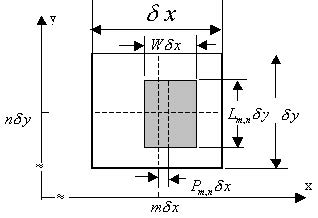
\includegraphics[width=0.35\textwidth]{img//chouyang.jpg}
			\caption{抽样单元的示意图}
			\label{chouyang}
		\end{figure}
		图\ref{chouyang}所示是采用矩形通光孔径编码的计算全息图的一个抽样单元的示意图。图中,$\delta x$和$\delta y$ 为抽样单元的抽样间隔,$W\delta x$为开孔的宽度,$L_{mn}\delta y$为开孔的高度,$P_{mn}\delta x$为开孔中心到抽样单元中心的距离。我们可以选取矩形孔的宽度参数$W$为定值,用高度参数$L_{mn}$和位置参数$P_{mn}$来分别编码光波场的振幅和位相。设待记录光波场的归一化复振幅分布函数为:
		\begin{equation}
			f_{mn}=A_{mn}\exp(j\phi_{mn})
		\end{equation}
		孔径参数和复振幅函数的编码关系为:
		\begin{equation}
			L_{mn}=A_{mn},\quad P_{mn}=\phi_{mn}/2\pi K
		\end{equation}
		利用这种方法编码的计算全息图的透过率只有0、1两个值,故制作简单,抗干扰能力强,对记录介质的非线性效应不敏感,可多次复制而不失真,因而应用较为广泛。

	\subsection{数字全息图的再现}
	随着数字全息技术的发展,出现了多种类型的数字全息图。从物光和参考光的位置是否同轴考虑,可以分为同轴数字全息图和离轴数字全息图;从记录时物体与全息图的相对位置考虑,可以分为菲涅耳数字全息图、夫琅禾费数字全息图和数字像面全息图。数字全息图的数值再现方式主要有两种:第一种是由计算机程序完成数字全息图的衍射及成像等过程,获得重构的物光光波场,再通过数字显示设备显示光波场的强度图像;第二种是由计算机程序对数字全息图进行简单处理,再借助液晶空间光调制器(Liquid crystals-Spatial light modulators, LC-SLM)、数字微镜(Digital Micromirror Device, DMD)等衍射成像设备来获得重构的物光光波场。

	从摄像机记录的光波场,到以数字形式存储全息图,再到数值再现全息图,数字全息技术的这一过程可以看作是一个数字化的相干光学成像系统,它能产生一个复波场,而这个复波场是经原始物体折射或衍射的像。对于这个成像系统,只要在物场给定一个输入函数,就能在像场得到一个输出函数。

	如图\ref{yuanli}所示,$x_Iy_I$面是数值再现的成像平面,与全息平面相距$d$,也称为再现距离。 $U_I(x_Iy_I)$是再现像的复振幅分布,因为它是一个二维复数矩阵,所以可以同时得到再现像的强度和相位分布。菲涅耳数字全息图再现过程就是一个菲涅耳衍射过程,根据衍射原理和再现距离可得再现平面上的光场分布,即:
	\begin{equation}
		\begin{aligned}
		&U_I(x_Iy_I)=\frac{\exp(jkd)}{j\lambda d}\iint_{-\infty}{\infty}I(u,v)C(u,v)\\ &\exp\{\frac{jk}{2d}(u^2+v^2)-\frac{i2\pi}{\lambda d}(ux_I+vy_I)\}dudv	
		\end{aligned}
	\end{equation}
	式中,$C(u,v)$是计算机模拟的再现光复振幅分布。在满足菲涅尔衍射条件下,$|d|$必须等于记录距离$d_0$。

	数字像面全息图是物光场的像与参考光在全息平面干涉的强度分布$I_H(x,y)$。因此$I(u,v)$的傅里叶变换频谱$I(f_u,f_v)$将包含原始物光波的频谱,同时存在物光共轭像的频谱及零级衍射光。如果利用频谱滤波或在参考光中引入相移等方法消除共轭像的频谱及零级衍射光,这样就将得到物光场在全息平面$xy$面上的像的频谱$I_o(f_u,f_v)$,再通过傅里叶反变换,就可以获得物光场的像的复振幅分布$U_I(x_I,y_I)$。
	
	容易看出,再现像的强度分布$I_I(x_I,y_I)$和相位分布$\Phi_I(x_I,y_I)$都可以由复振幅分布$U_I(x_I,y_I)$计算得到:
	\begin{equation}
	\begin{aligned}
		&I_I(x_I,y_I)=U_I(x_I,y_I)U_I^*(x_I,y_I)\\
		&\Phi_I(x_I,y_I)=\arctan\frac{ImU_I(x_I,y_I)}{Re U_I(x_I,y_I)}
	\end{aligned}
	\end{equation}

	\subsection{空间光调制器实时再现}
	图\ref{yejing}中液晶屏两侧的起偏器和检偏器相互平行,自然光透过起偏器后变为线偏振光偏振方向为水平。右侧V=O,不加电压,液晶分子自然扭曲90°,透过光14的偏振方向也旋转90°,与检偏器方向垂直,无光线射出,即为关态。然而在左侧V$\not=$0,分子沿电场方向排列,对光的偏振方向没有影响,光线经检偏器射出,即为开态。这样即实现了通过电压控制光线通过的功能。

	利用空间光调制器来代替传统全息干板,可以实现传统全息实验中无法实现的实时全息功能。但由于液晶空间光调制器的分辨率比干板的低,当有参考光照射空间光调制器时衍射过程中物的振幅信息和相位信息都会有丢失,所以在记录全息图的时候我们一定要尽可能获得较完备信息。同时为提高再现信息质量,物体尺寸、记录距离、参物光干涉夹角以及共轭像的分离都可以作为实验中的优化参数。
	\begin{figure}[H]
		\centering
		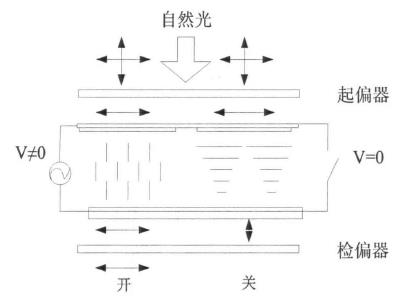
\includegraphics[width=0.4\textwidth]{img//yejing.jpg}
		\caption{空间光调制器}
		\label{yejing}
	\end{figure}

	\section{计算机模拟的数字全息记录实验}
		使用根据上文所述的计算模拟全息的记录原理编写好的全息实验程序,可以把原始图片的模拟全息结果给出。使用“菲涅尔全息图数字模拟”程序,可以得到如下的结果:图\ref{digpara}为模拟参数,图\ref{sample}为原始图像,图\ref{holo1}为得到的模拟全息图。

		\begin{figure}[H]
			\centering
			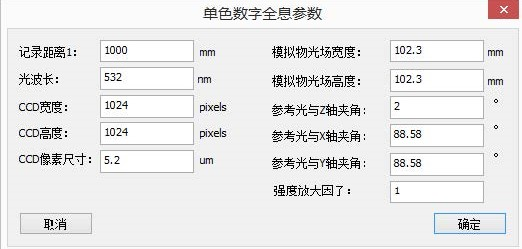
\includegraphics[width=0.4\textwidth]{img//eq0.jpg}
			\caption{计算模拟数字全息参数}
			\label{digpara}
		\end{figure}

		\begin{figure}[H]
			\centering
			
\includegraphics[width=0.3\textwidth]{img//1.1.jpg}
			\caption{计算模拟的原始图片}
			\label{sample}
		\end{figure}

		\begin{figure}[H]
			\centering
			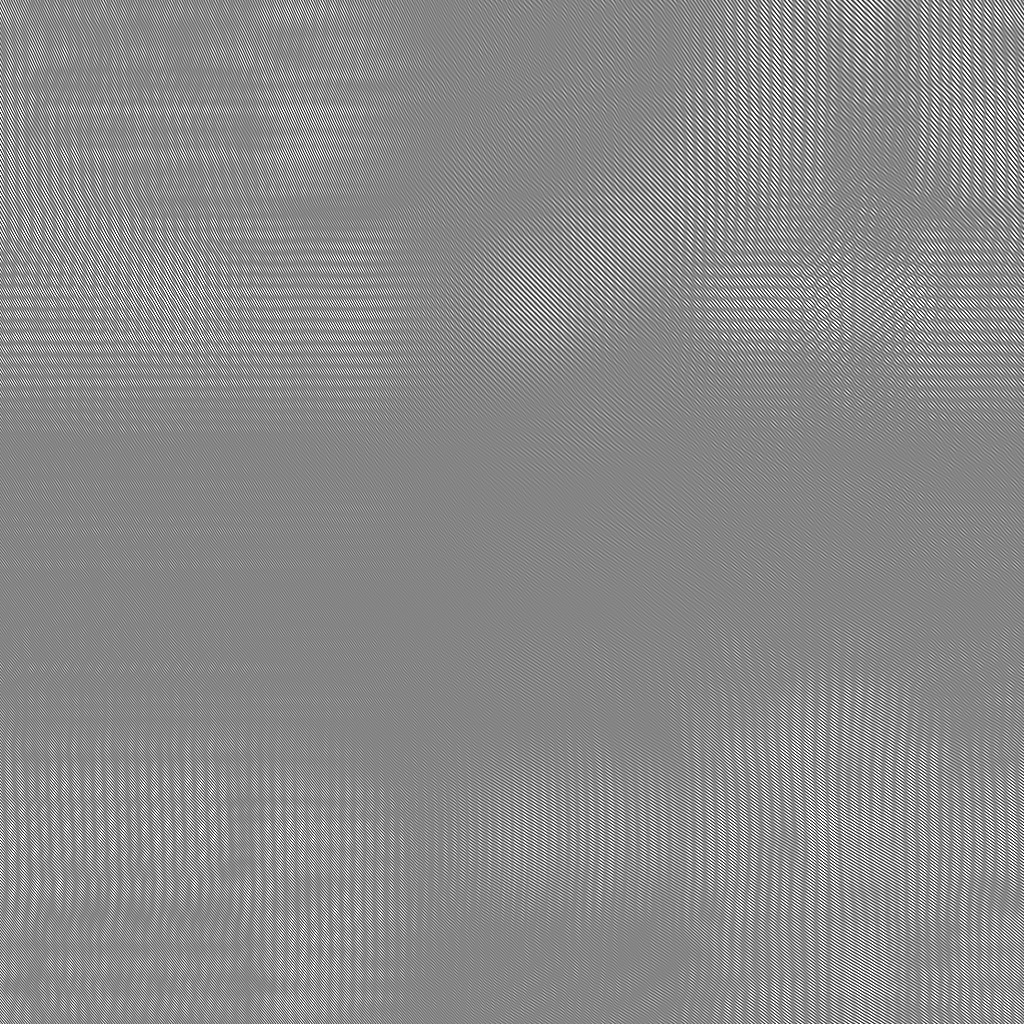
\includegraphics[width=0.3\textwidth]{img//1.2.jpg}
			\caption{图\ref{sample}的计算模拟全息图}
			\label{holo1}
		\end{figure}

	\section{光学方法实现数字全息记录}

		\subsection{实验光路}
		(1)透射数字全息获得可以通过搭建马赫曾德干涉光路获得全息图。调节光路,根据图\ref{eq1show}透射光路示意图将激光器、扩束准直系统、分束镜、反射镜以及	合束镜,使各元件等高同轴。
		\begin{figure}[H]
			\centering
			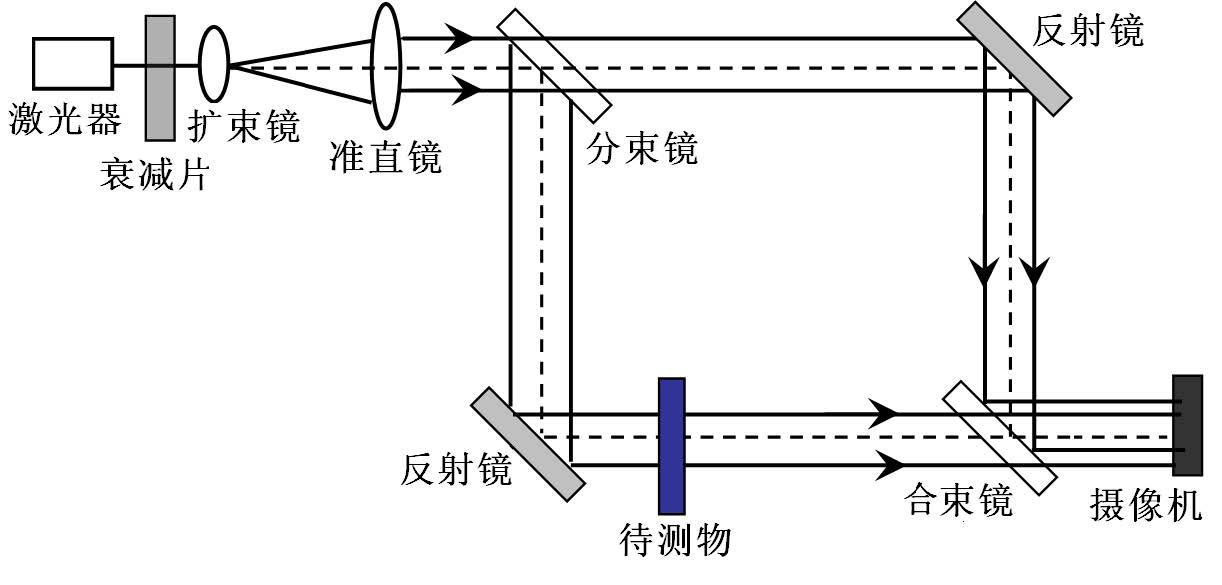
\includegraphics[width=0.45\textwidth]{img//eq11.jpg}
			\caption{光学全息记录光路示意图}
			\label{eq1show}
		\end{figure}
		\begin{figure}[H]
			\centering
			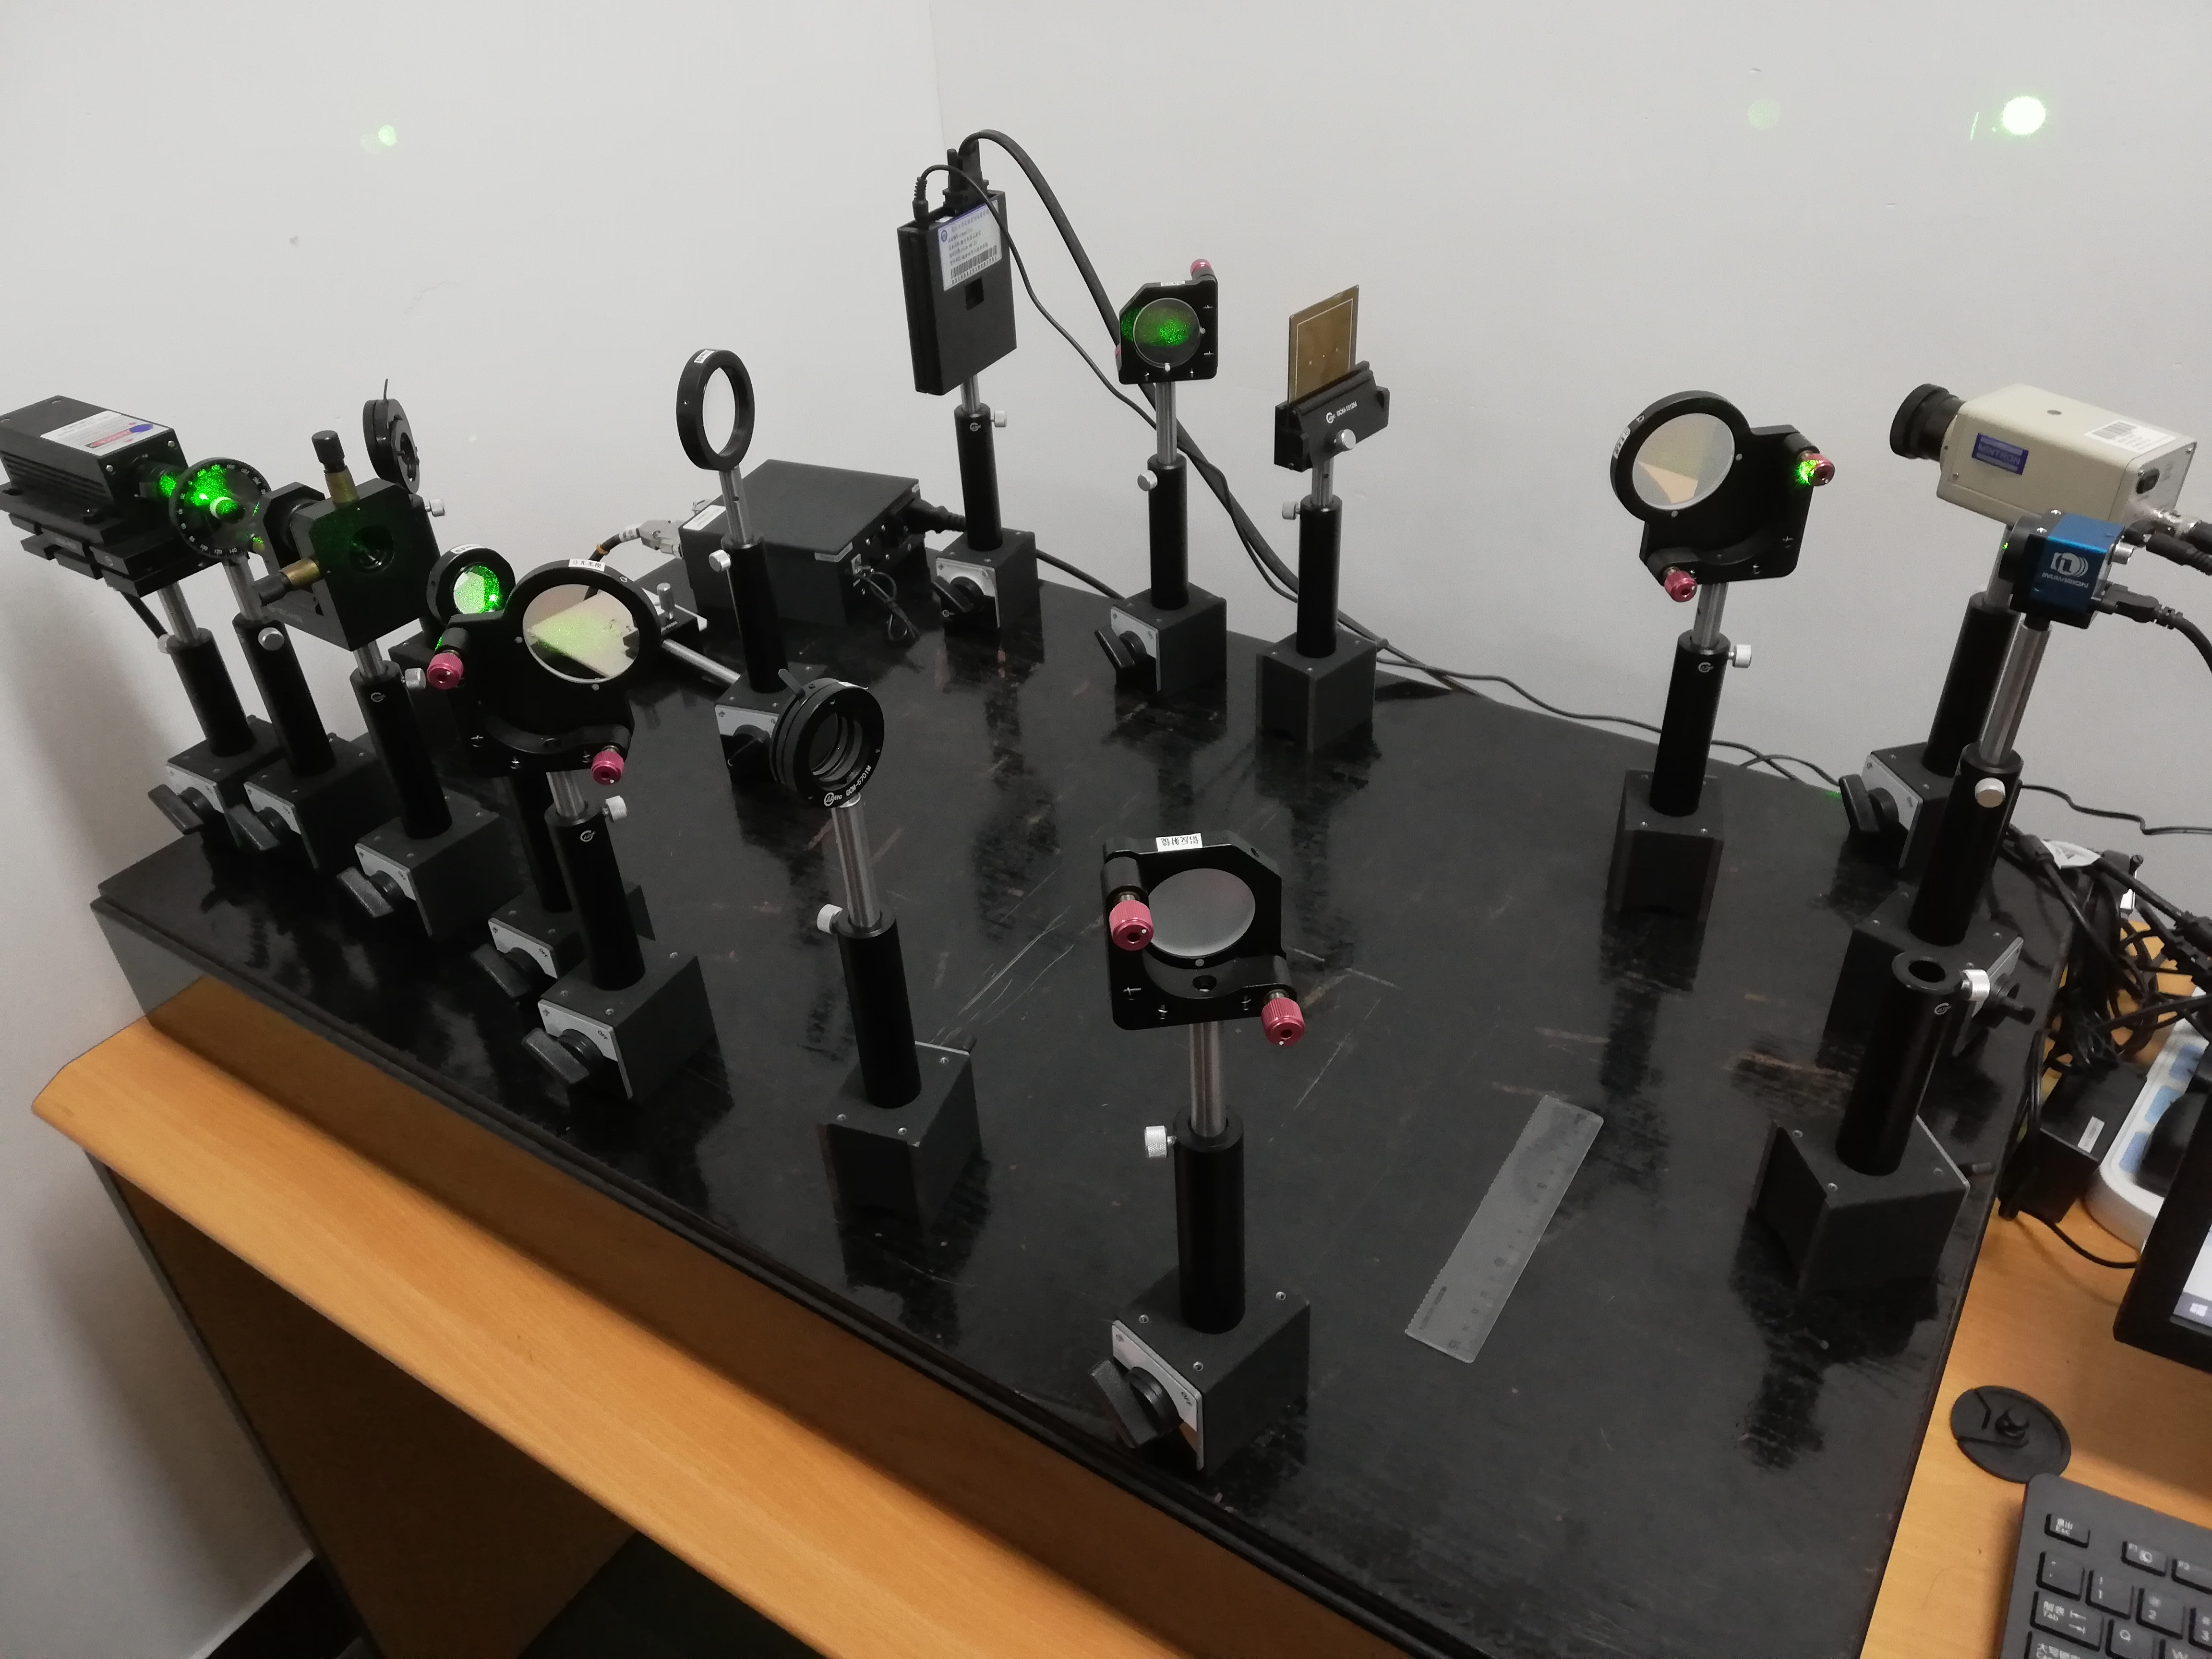
\includegraphics[width=0.45\textwidth]{img//eq1.jpg}
			\caption{光学全息记录实验光路实物图}
			\label{eq1}
		\end{figure}

		(2)通过调整合束镜。可以改变条纹疏密,待条纹较密但人眼仍可分辨时即可。

		(3)摄像机与待测物的距离可有公式$\Delta L_0=\lambda d/p$确定,式中$\Delta L_0$为物体尺寸的 4 倍,$\lambda$是光波长,$d$ 为记录距离,$p$ 为 CCD 的像元尺寸。 其中再现距离长短一是影响再现物的大小,一是影响±1 级像与 0 级分开程度;条纹疏密主要影响	±1级像与级像与0级分开程度,条纹越密分开角度越大,条纹越疏分开角度越小。例如:物体尺寸选如:物体尺寸选27mm,CCD像素选像素选5.2um,光波长用,光波长用632.8nm,则记录距离应该则记录距离应该选大于选大于854mm。。由于实验过程中使用的激光波长是由于实验过程中使用的激光波长是532nm,所以记录距离可选,所以记录距离可选择择150mm—450mm。

		(4)调整摄像机的快门速度和增益 获得一定灰度的全息,一般来讲,物光和参考光光强相近,单独一束光的灰度大于 25 即可。例如,确定快门速度为 100微秒, 调整可调圆形衰减器即可获得合适灰度。
		
		(5)经摄像机采集后可获得大小为 1024*1024 的全息图,将全息图通过数字全息软件便可恢复原物信息。

		\subsection{光学记录得到的数字全息图}

		分别使用“大”、“恒”字光栅作为物光,可以得到其数字全息图如下所示:

		\begin{figure}[H]
			\centering
			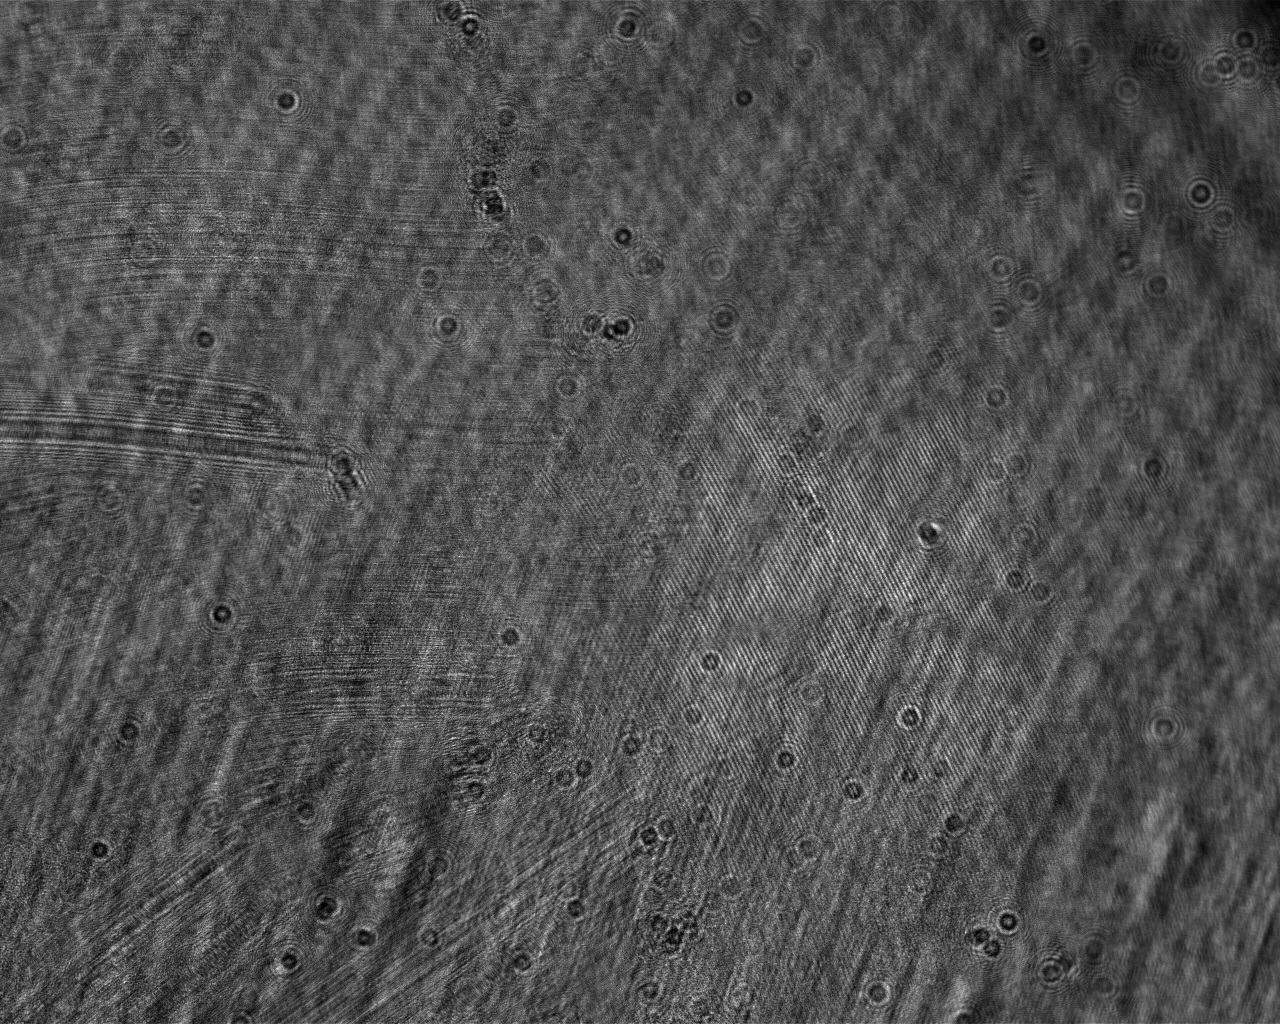
\includegraphics[width=0.35\textwidth]{img//2.5.3.jpg}
			\caption{“大”字光学记录方法得到的数字全息图}
			\label{holo2}
		\end{figure}
		\begin{figure}[H]
			\centering
			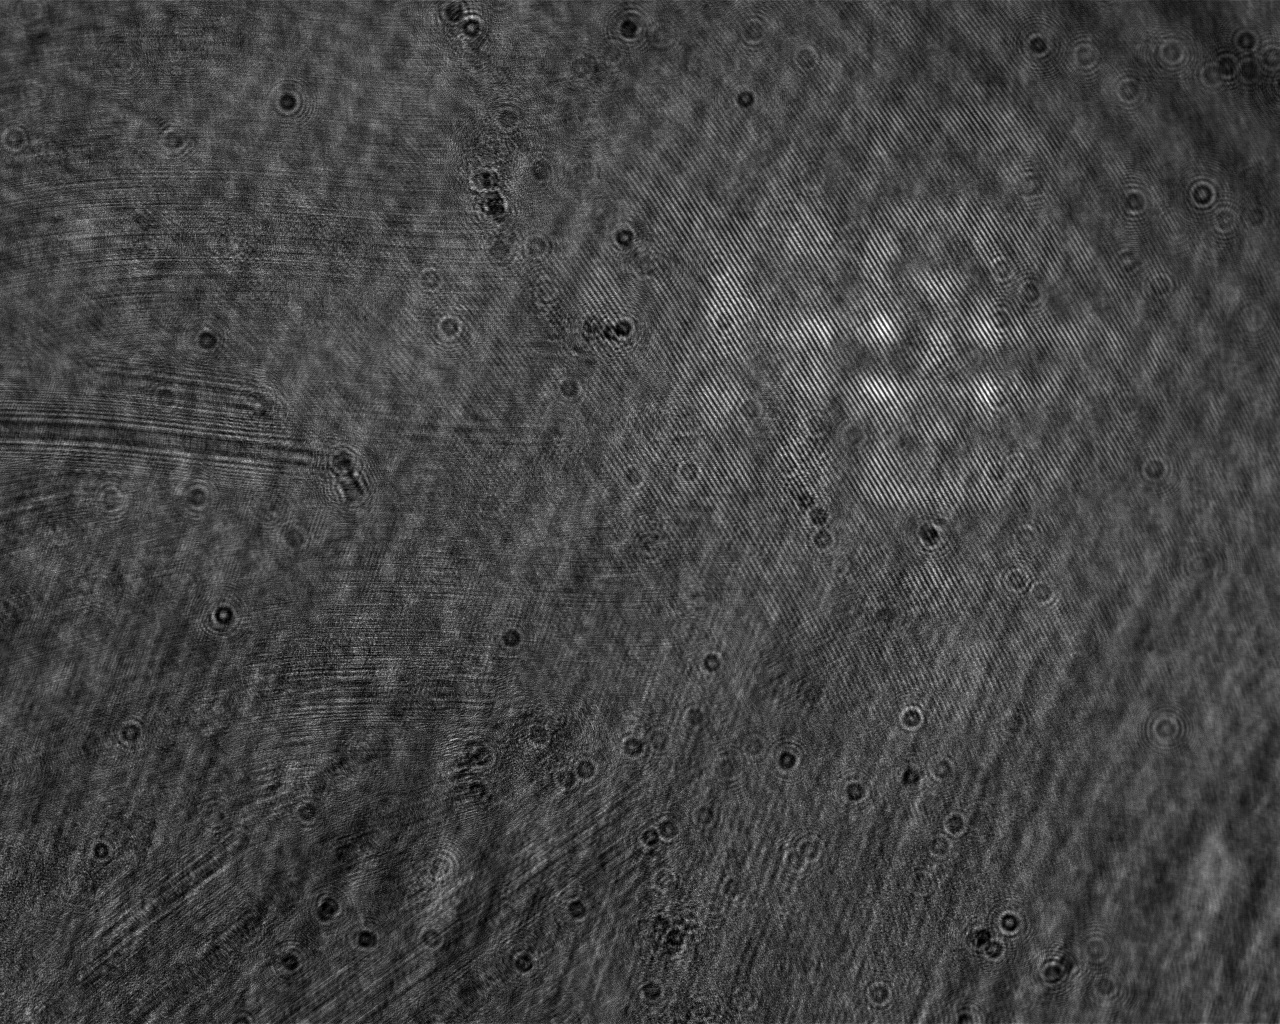
\includegraphics[width=0.35\textwidth]{img//2.4.7.jpg}
			\caption{“恒”字光学记录方法得到的数字全息图}
			\label{holo3}
		\end{figure}

	\section{计算机模拟的数字全息再现}
		使用“一步菲涅尔全息数字重现”程序,使用和记录全息图时相同的参数,就可以获得重建图像的结果。我们把计算机模拟得到的全息图、通过光学方法得到的全息图分别使用该程序进行模拟重现,可以得到如下的结果。

		\subsection{模拟再现结果}
		对于图\ref{holo1}的模拟全息图,使用程序计算模拟得到的重现结果如图\ref{holorel1}所示。

		\begin{figure}[H]
			\centering
			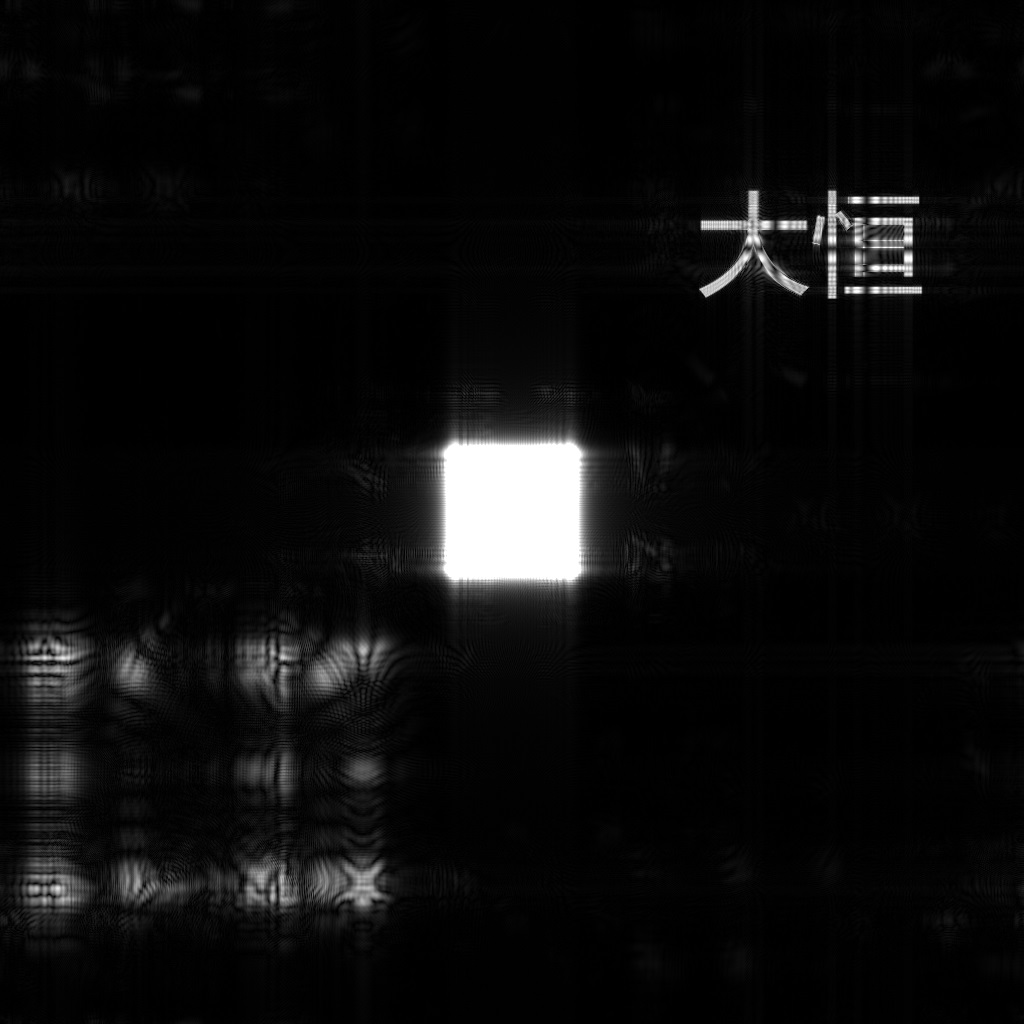
\includegraphics[width=0.35\textwidth]{img//1.3.jpg}
			\caption{图\ref{holo1}的模拟全息重现图}
			\label{holorel1}
		\end{figure}

		对于光学方法得到的数字全息图,我们通过测量记录距离,将该参数输入程序并进行重建,可以得到他们的模拟全息重建图。使用程序计算模拟得到的“大”、“恒”的全息重现结果如图\ref{holorel2}和图\ref{holorel3}所示。
		\begin{figure}[H]
			\centering
			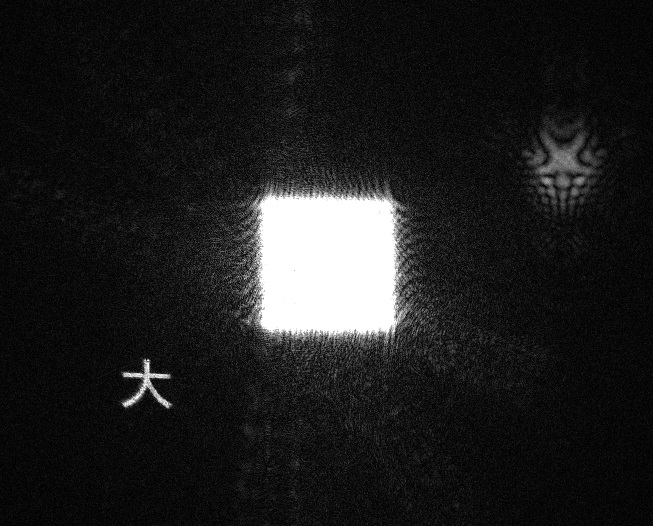
\includegraphics[width=0.35\textwidth]{img//2.5.3.1.jpg}
			\caption{图\ref{holo2}(“大”字)的模拟全息重现图}
			\label{holorel2}
		\end{figure}

		\begin{figure}[H]
			\centering
			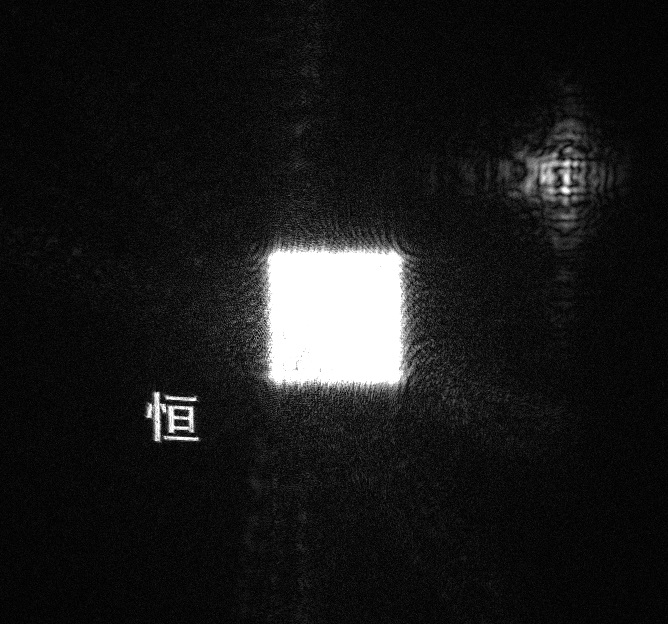
\includegraphics[width=0.35\textwidth]{img//2.4.7.1.jpg}
			\caption{图\ref{holo3}(“恒”字)的模拟全息重现图}
			\label{holorel3}
		\end{figure}

	\section{光学方法实现数字全息再现}
		使用空间光调制器,可以把全息图加载到光路中,从而用光学方法实现全息图的再现。

		\subsection{实验光路}
		搭建图\ref{eq2show}所给光路,依次调整激光器、扩束系统、准直系统、空间光调制器、凸透镜和摄像机,保证各器件同轴等高, 凸透镜可紧挨空间光调制器。当再现光源入射到空间光调制器上 调整圆形可调衰减器和摄像机的采集时间, 在 摄像机 上可以看到再现像,调整凸透镜与空间光调制器的距离能改变再现像的大小。
		\begin{figure}[H]
			\centering
			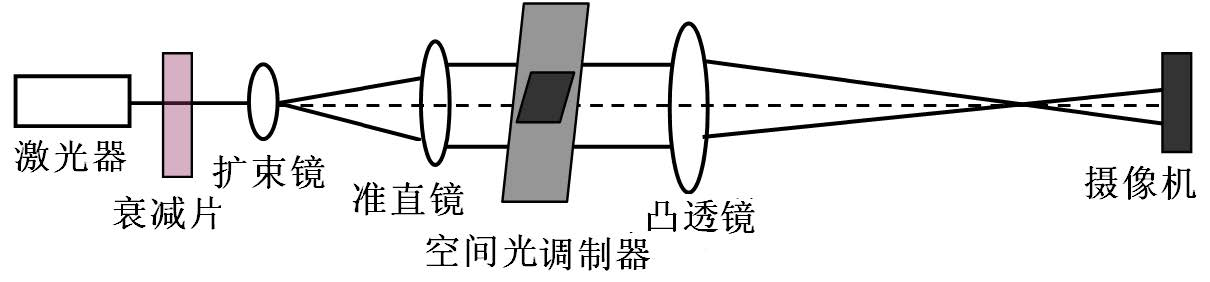
\includegraphics[width=0.45\textwidth]{img//eq22.jpg}
			\caption{光学全息重现光路示意图}
			\label{eq2show}
		\end{figure}
		\begin{figure}[H]
			\centering
			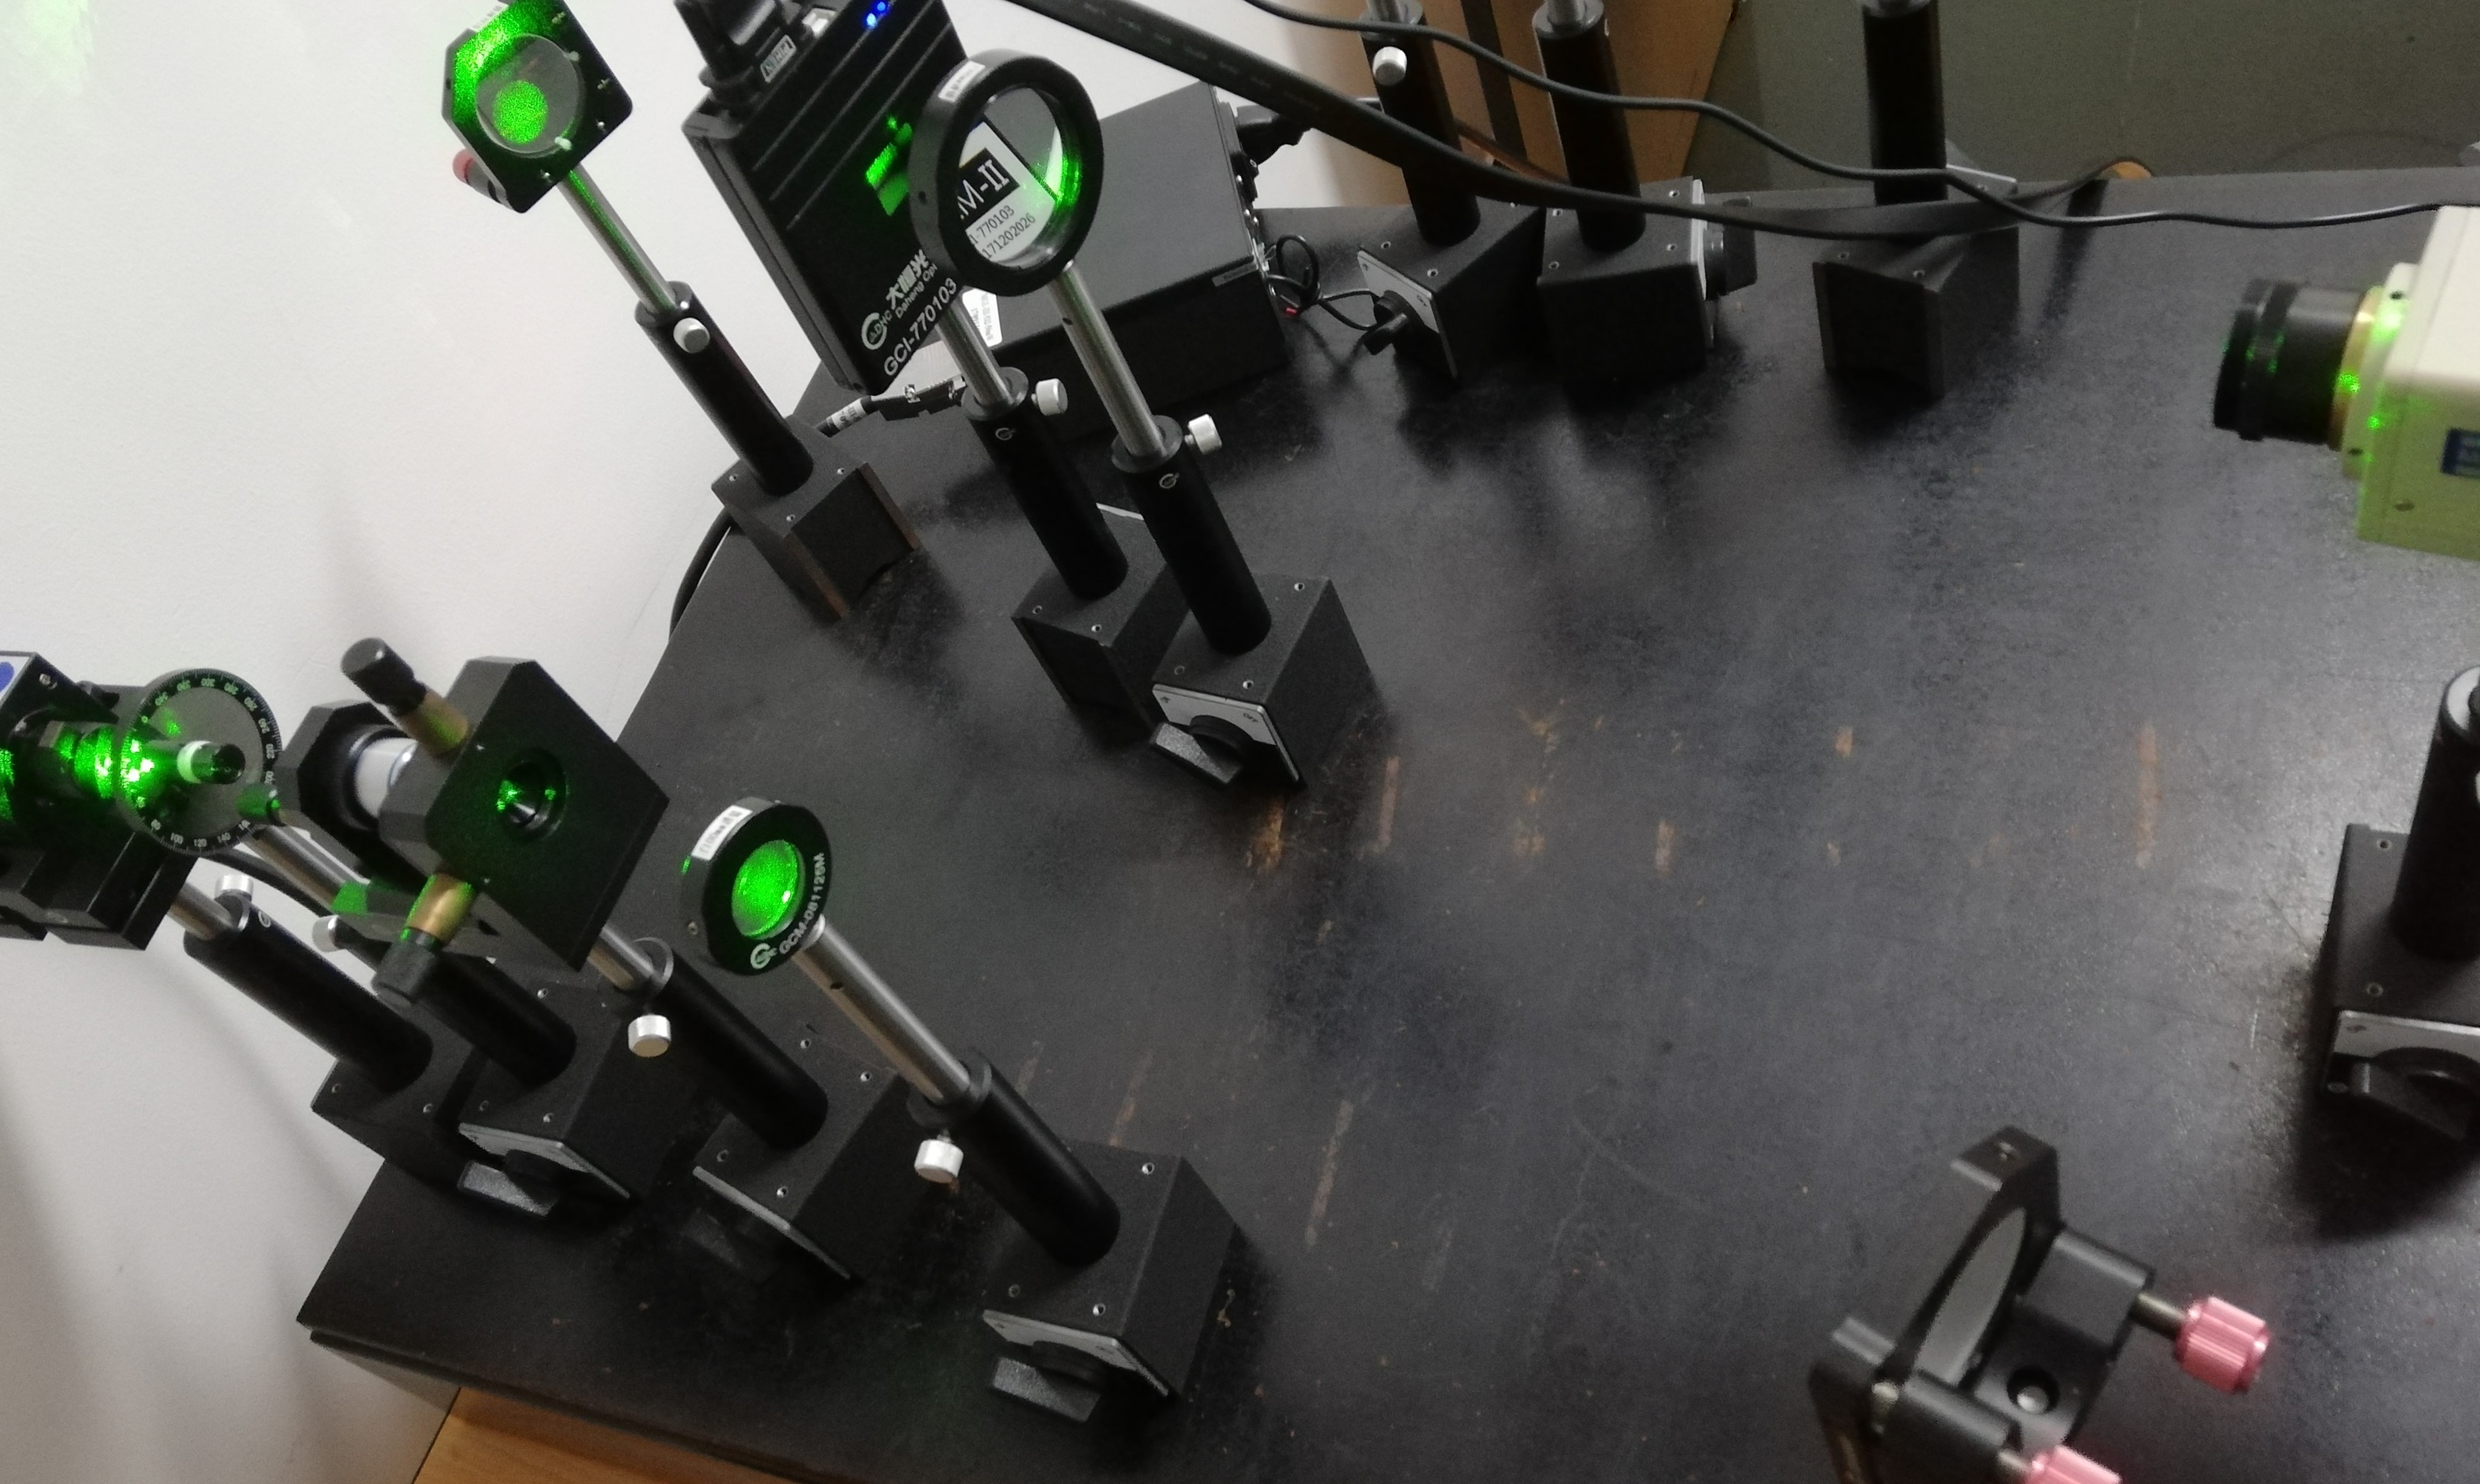
\includegraphics[width=0.45\textwidth]{img//eq2.jpg}
			\caption{光学全息重现实验光路(左上、右下角为使用反射镜将光路扩展)}
			\label{eq2}
		\end{figure}

		\subsection{光学再现结果}
		本别把计算模拟得到的全息图、光学方法拍摄的全息图加载到空间光调制器上, 使用CCD可以在像的位置得到全息图的再现结果。

		图\ref{holorel11}是计算模拟的到的“大恒”全息图的重现结果:
		\begin{figure}[H]
			\centering
			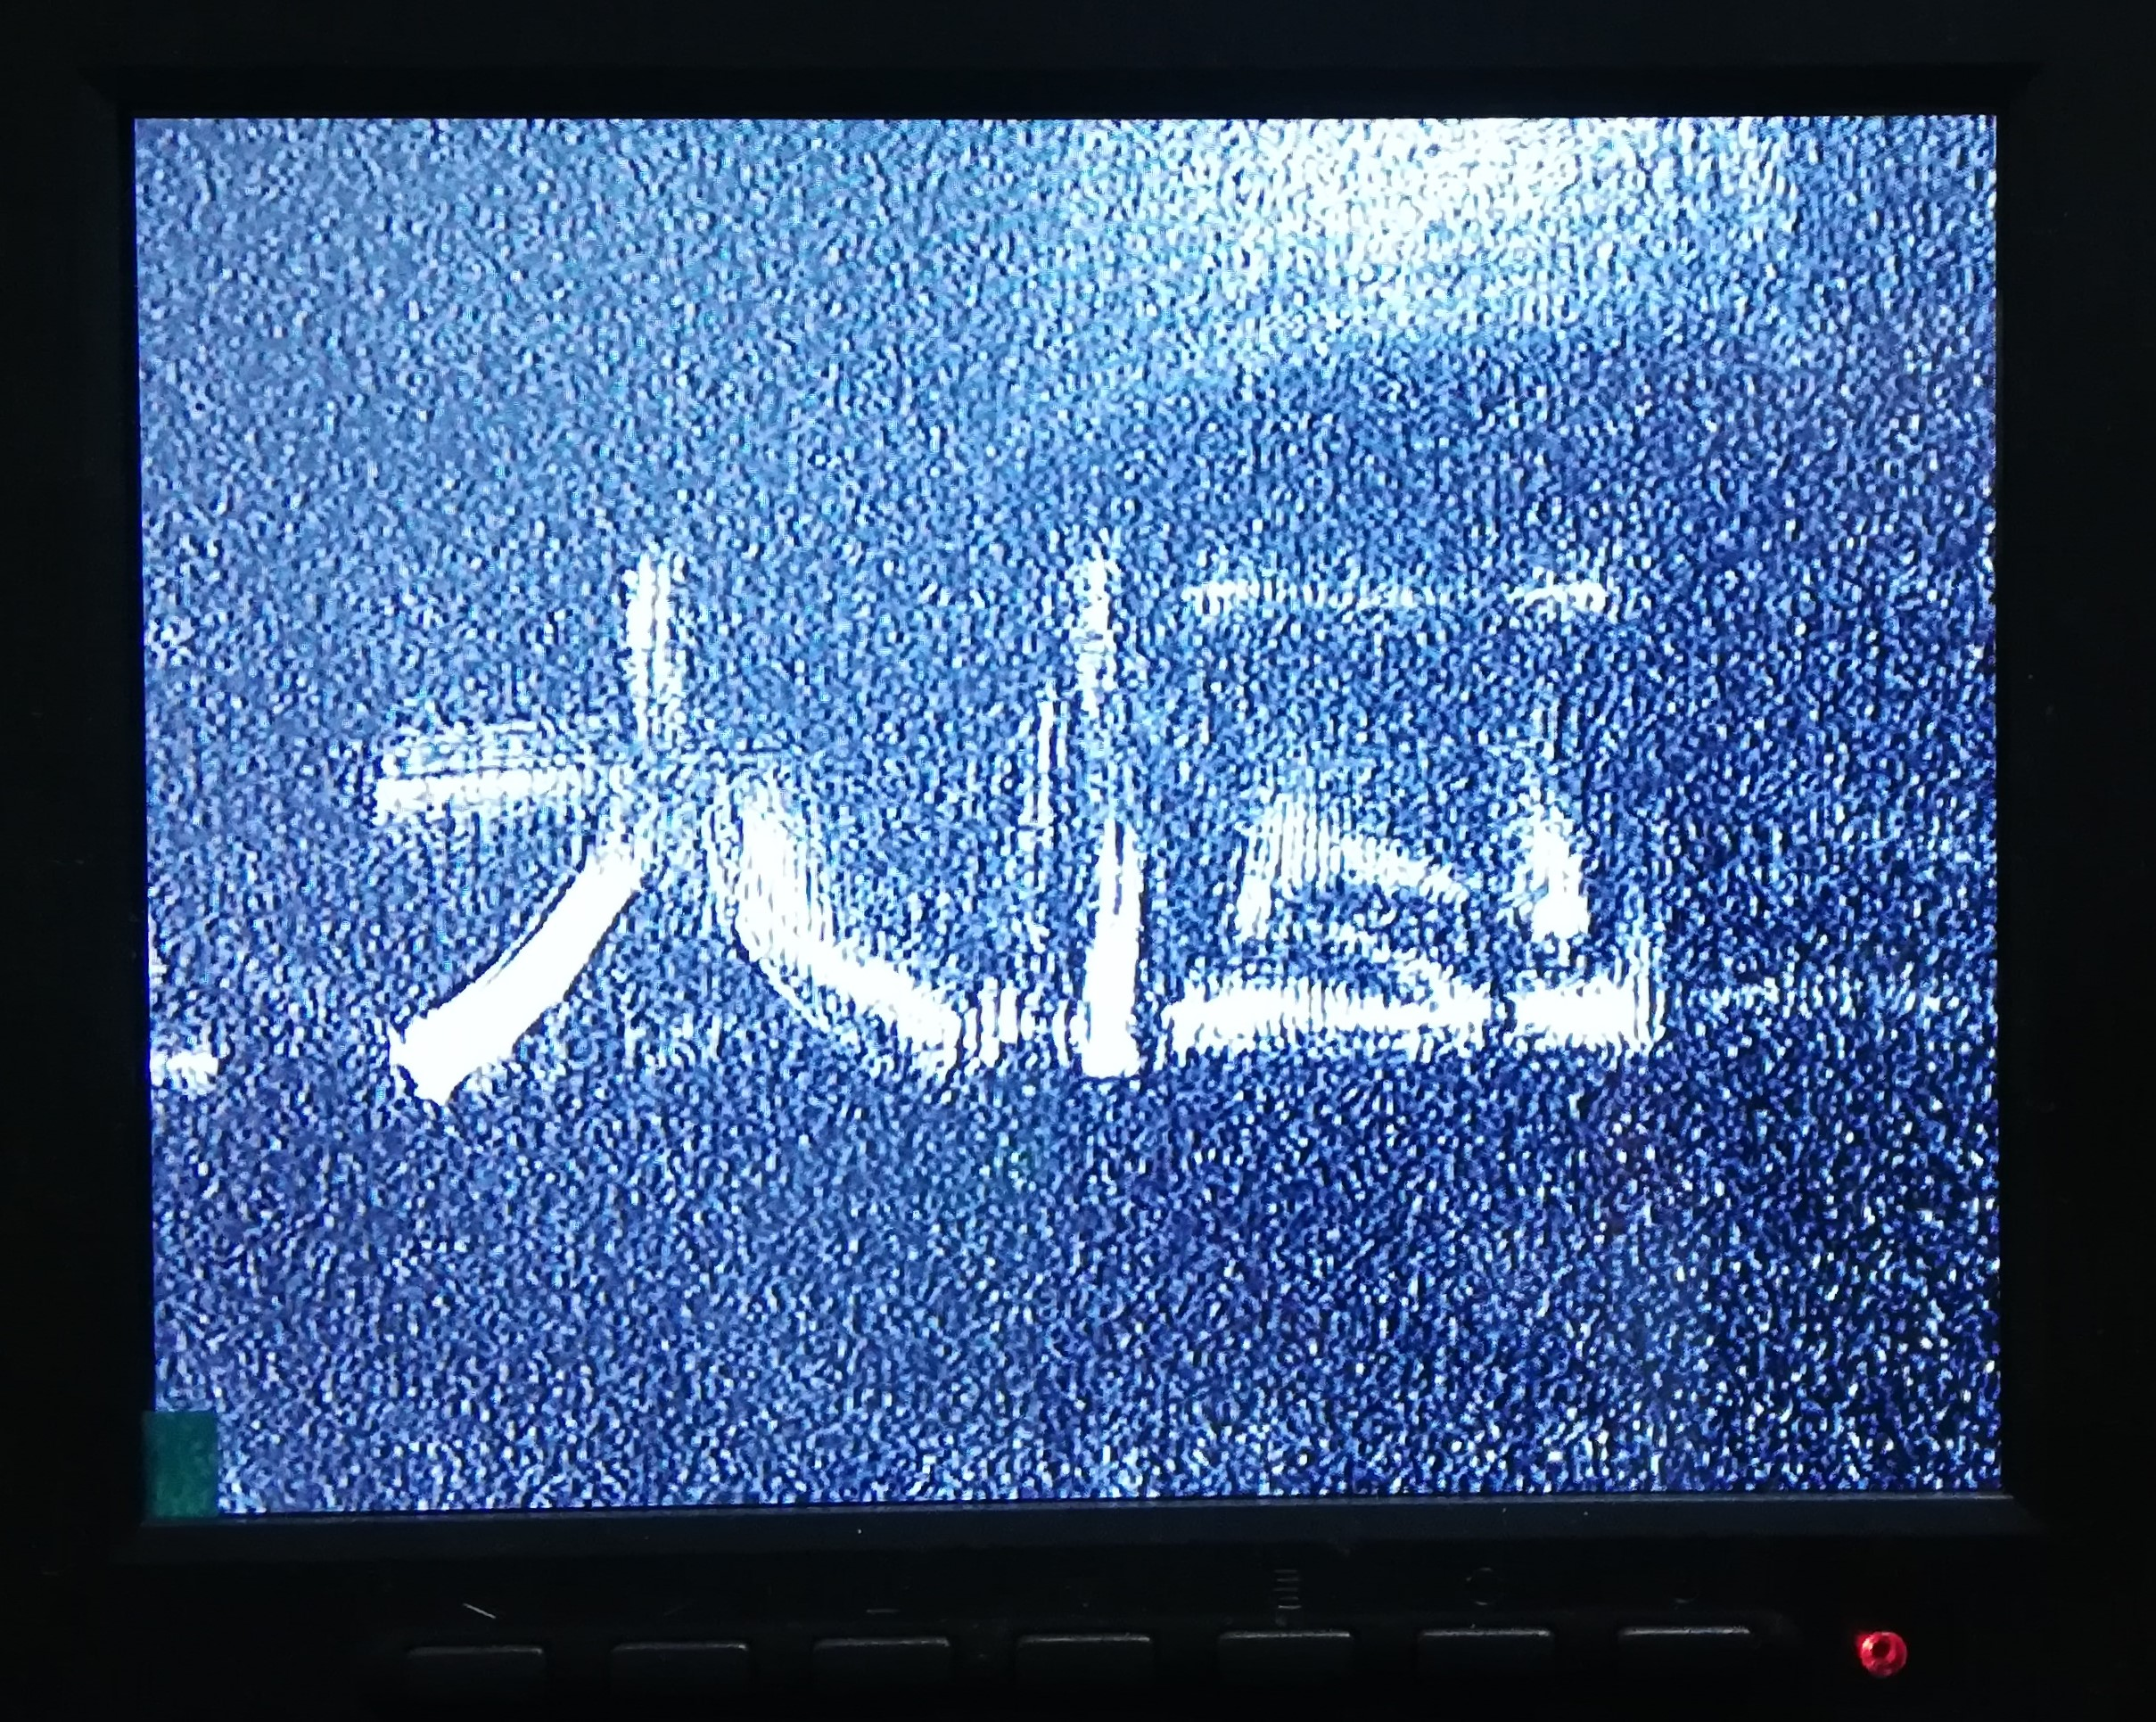
\includegraphics[width=0.35\textwidth]{img//1.4.jpg}
			\caption{图\ref{holo1}的光学全息重现图}
			\label{holorel11}
		\end{figure}

		图\ref{holorel22}、图\ref{holorel33}分别是光学方法拍摄的“大”、“恒”字的数字全息图的重现结果:
		\begin{figure}[H]
			\centering
			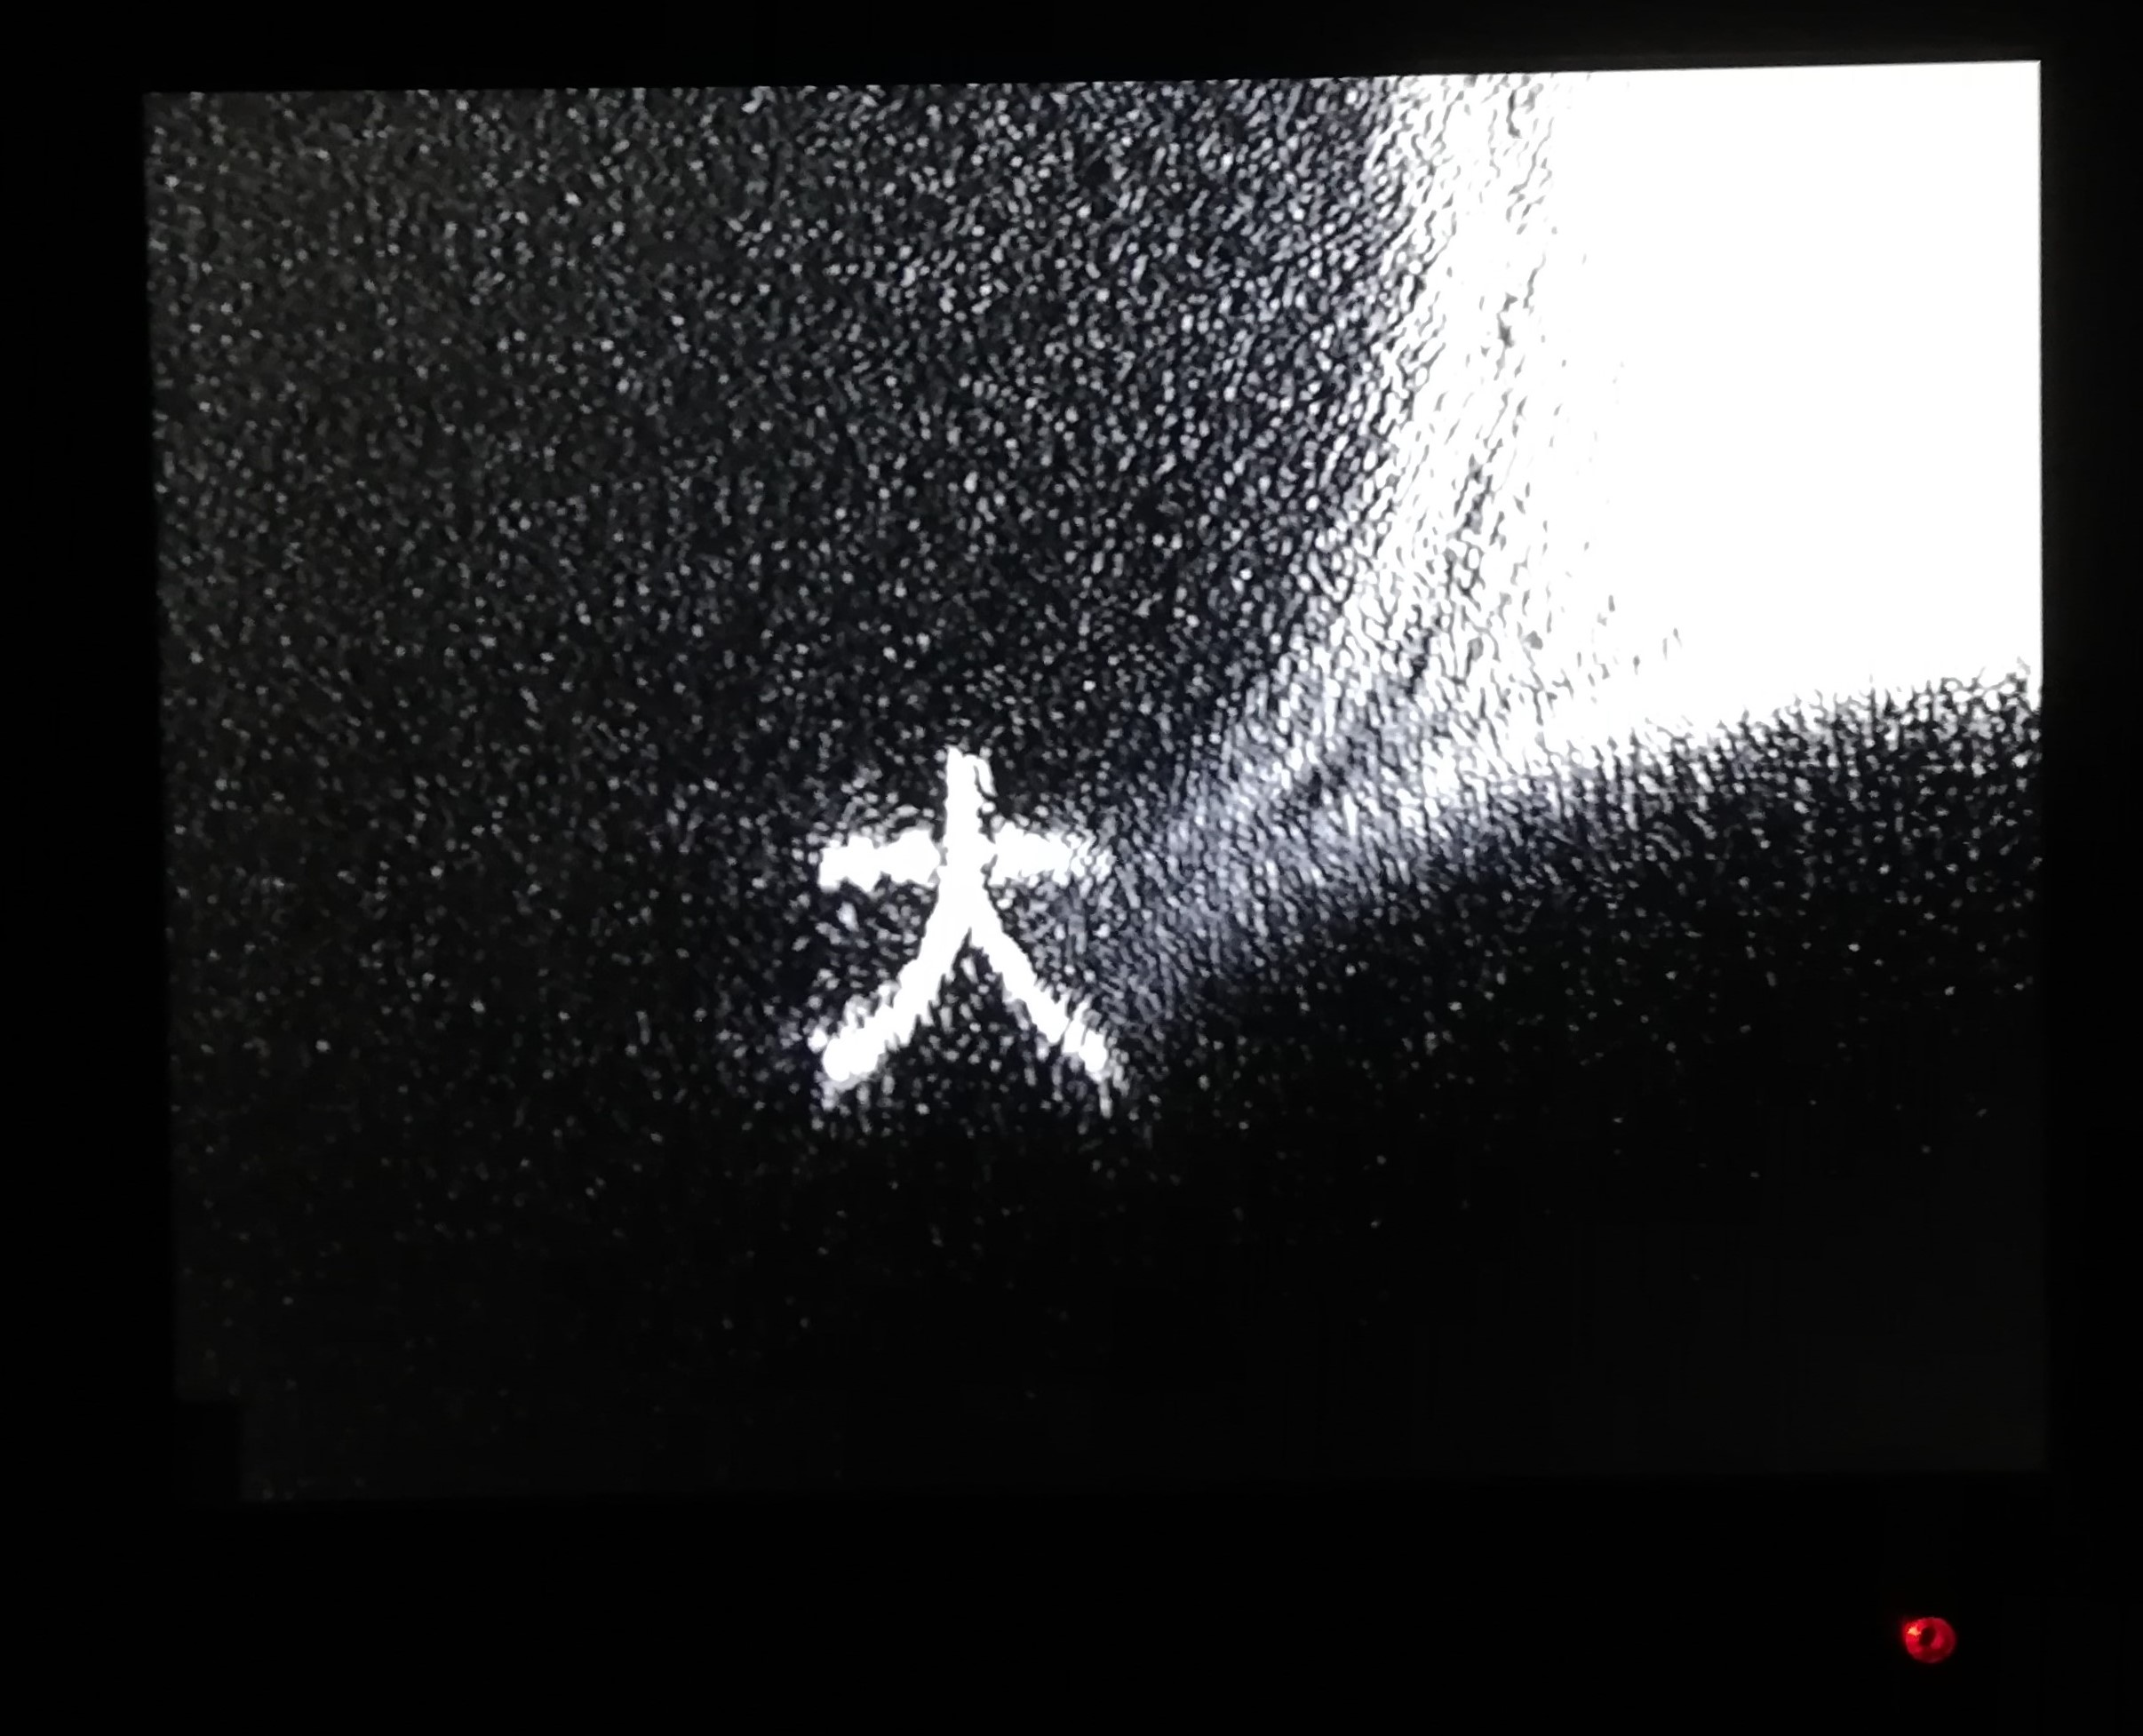
\includegraphics[width=0.35\textwidth]{img//2.5.3.2.jpg}
			\caption{图\ref{holo2}(“大”字)的光学全息重现图}
			\label{holorel22}
		\end{figure}
		\begin{figure}[H]
			\centering
			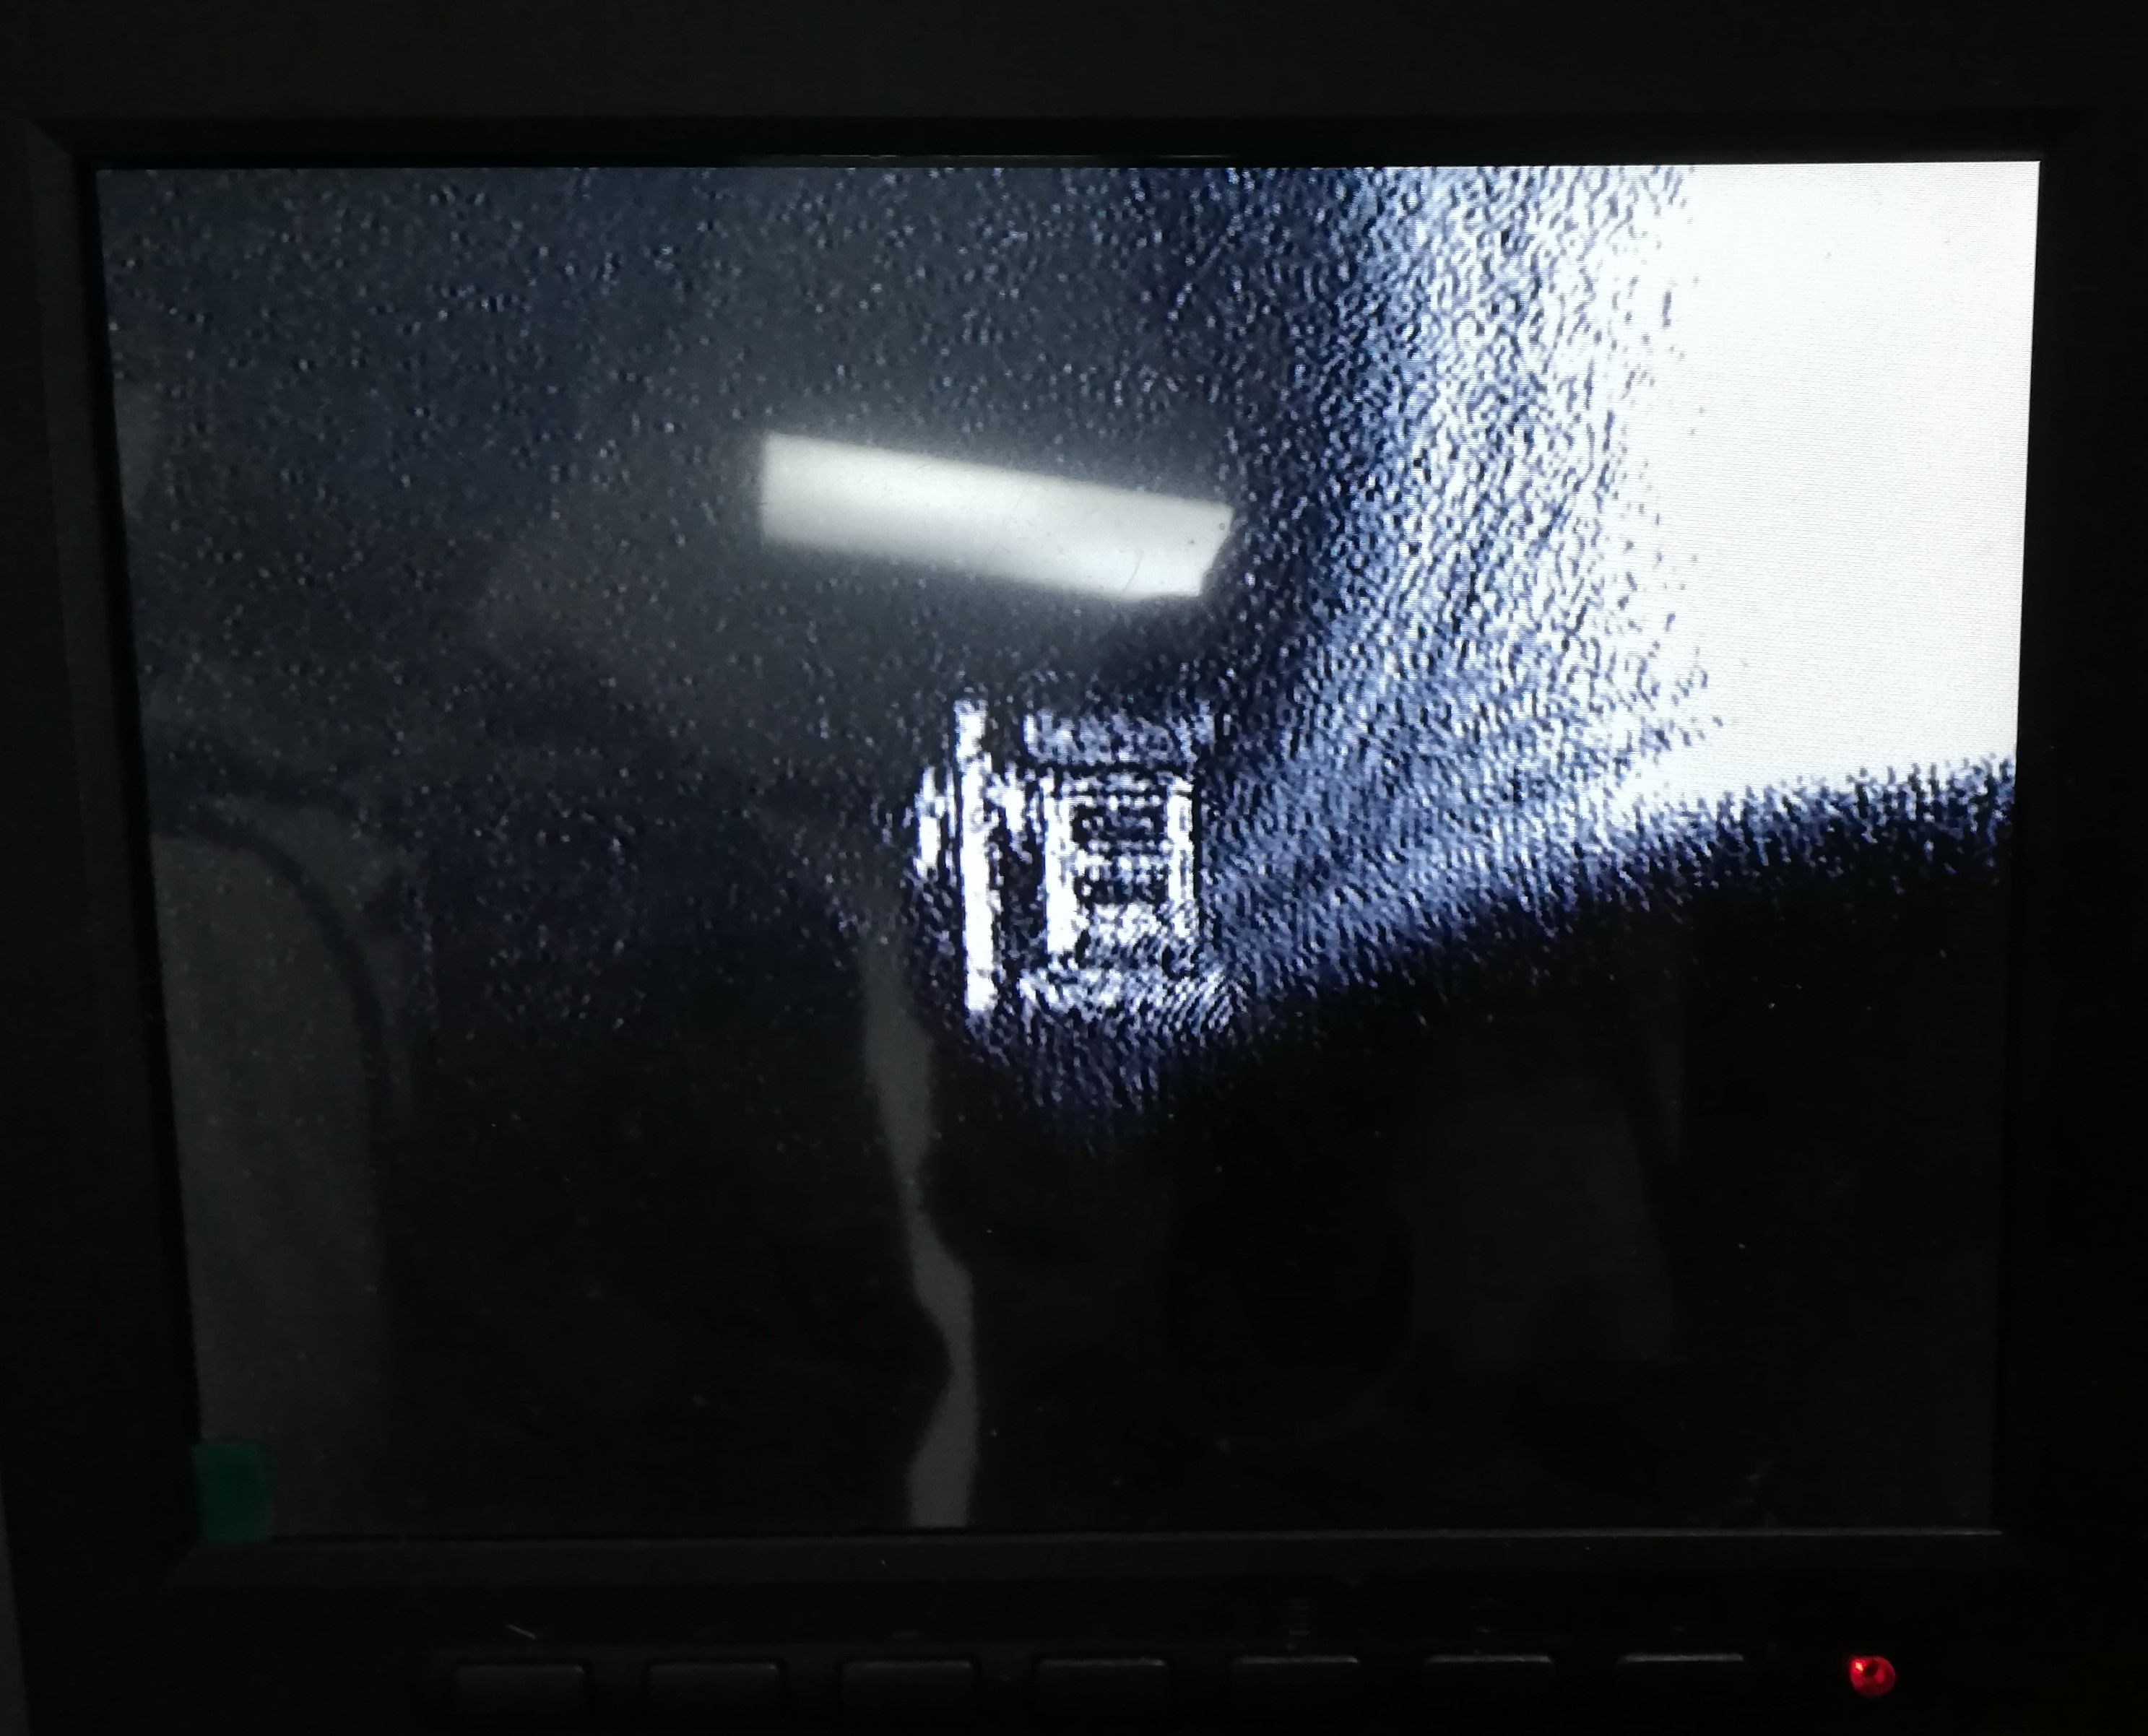
\includegraphics[width=0.35\textwidth]{img//2.4.7.3.jpg}
			\caption{图\ref{holo3}(“恒”字)的光学全息重现图\quad (“恒”字上方是屏幕反射的灯光)}
			\label{holorel33}
		\end{figure}


	\begin{thebibliography}{9}
		\bibitem{1} 赵凯华. 光学[M]. 北京:北京大学出版社, 1984, 2006.
		\bibitem{2} 古德曼. 傅里叶光学导论[M]. 北京:电子工业出版社, 2016.
		\bibitem{3} 黄威龙,白欣,梁海坤,梁绮霞,曾育锋.数字全息光学实验探究及再现清晰度优化[J].物理实验,2019,39(04):44-48.
		\bibitem{4} 肖体乔,徐至展,陈建文,朱佩平,寇雷刚,程亚.全息图的数字重现[J].光学学报,1995(02):129-134.

	\end{thebibliography}
	
% %\newpage
% %换一栏,而不是换一页。换一页用\clearpage
% \section{温度测控原理}
% 温度的测控,包含温度的测量和控制,其中温度的测量往往转化为电信号输出,而温度的控制通常使用电磁继电器实现。本实验设计的温度测控仪器主要包括两个部分,一个是温度传感器,另一个是温度测控电路。

% 	\subsection{温度测控仪电路}
% 		%%subsection:第二级,小节,2.1
% 	基于以上三种温度测控仪,我们相应得也有三种温度测控仪电路。
% 		%%subsection后面的正文:自动换段,正常缩进
% 	\subsubsection{基于 AD590 电流型温度传感器的数显温度测控仪}
% 		%%subsubsection: 第三级,小小节,2.1.1
% 	这里本来并不需要文字。
% 		%%subsubsection后面的正文:自动换段,正常缩进
% 	\paragraph{A.温度显示原理}
% 		%%paragraph: 大段落,加粗,不缩进
% 	如果就需要这样的效果,那很好。
% 	\paragraph{B.温度控制原理}但段落后面如果需要换行,就是个棘手的问题。
% 		%%paragraph后面的正文:无论是紧接着}敲还是换了几行,都会空一到两格后直接跟在后面。
% 	\subparagraph{第一步:调零。}小段落后面的正文也是一样,
% 		%%subparagraph:小段落,加粗,正常缩进
% 	\subparagraph{第二步:确定电压灵敏度}
% 	紧跟着段落标题。
% 		%%subparagraph后面的正文:无论是紧接着}敲还是换了几行,都会空一到两格后直接跟在后面。


% 	\subsection{温度传感器}
% 	本实验涉及三种温度测控仪的组装,分别采用三种不同的温度传感器,包括
% 	%%paragraph后面的换段方法
% 	\paragraph{(1)金属电阻温度传感器}~
% 		% ~是一个控制符号,不会真的输出~,而是空一格。
% 	\newline %换行,强制换行之后需要手动缩进,用命令\indent
% 	\indent 如 PT100 或 Cu50, PT100 即铂金属电阻,在 0℃时的电阻值为 $R_0=100\Omega$; Cu50 即铜金属电阻, 在 0℃时的电阻值为$R_0=50\Omega$。


% 	\subsection{实验内容}
% 	本实验中笔者选择了“基于LM35电压型温度传感器的数显温度测控仪”电路进行搭建和测试。
% 	%%自定义项目符号之(1)(2)(3)
% 	\begin{enumerate}[(1)]
% 		\item 根据图5搭建电路。
% 		\item 测量数字电压读数与温度之间的对应关系, 作电压与温度关系曲线。
% 	 	\item 利用组装的温度测控仪电路,将加热阱的温度控制在 75$^{\circ}C$。
% 	\end{enumerate}

% %%end------------------层级结构------------------------%%

% %%begin------------------插入图表------------------------%%

% \section{温度测控仪的搭建和测试}

% 	\subsection{测试用设备}
% 	\paragraph{A.其他设备}~
% 	\newline
% 	\indent 直流稳压电源用于提供测控仪电路的±12V电源,数字万用表的直流电压测量功能可用于替代数字电压表,用于指示温度测控仪的当前温度。各仪器使用方法请查阅教材。

% %%% 1 不跨栏单幅图
% 	% 图片的大小需要细细得调。需要掌握latex里面的长度单位和限制大小方法。
% 	\begin{figure}[H]
% 		\centering
% 		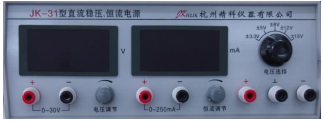
\includegraphics[width=0.5\textwidth]{img//device_3.png}
% 			%textwidth:正文宽度。双栏,则将两栏正文宽度相加。
% 		\caption{直流稳压电源}
% 		\label{powersource}
% 	\end{figure}

% %%% 2 跨栏单幅图
% 	% 在figure之右加上*即可。
% 	\begin{figure*}[H]
% 	\centering
% 	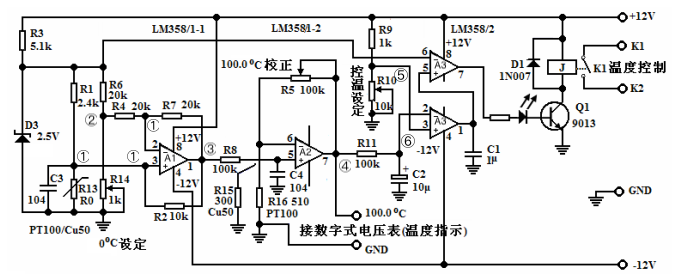
\includegraphics[width=1\textwidth]{img//Diagram_Cu50.png}
% 	\caption{基于 PT100(或 Cu50)温度传感器的数显温度测控仪}
% 	\label{Diagram_Cu50}
% 	\end{figure*}

% 	\paragraph{B.温度控制设备}~
% 	\newline

% %%% 3 两幅图并行排版,各有图题,还有一个总的图题
% 	% (1)注意正文中引用图片的方法
% 	% (2)不仅需要调节大小,还需要细细调节位置。通过{minipage}后面的补充参数来调节位置。图片大小最好用高度来调,并保证两个图高度一样。
% 	\indent 图\ref{fig:improved_subfig_a}为致冷/加热温度控制仪,从左到右分成三个部分,分别为(1)数字电压表(有20V和2V两个量程);(2)加热和致冷功率控制器;(3)温度设置和测量装置风扇用于加快空气流动。
% 	图\ref{fig:improved_subfig_b}的控温阱分为致冷阱和加热阱两种。制冷阱用于0℃至室温范围的实验,加热阱用于室温-100℃范围。

% 	\begin{figure*}[H]
% 		\centering
% 		\subfloat[致冷/加热温度控制仪]{
% 		\label{fig:improved_subfig_a}
% 		\begin{minipage}{0.5\textwidth}
% 			\centering
% 			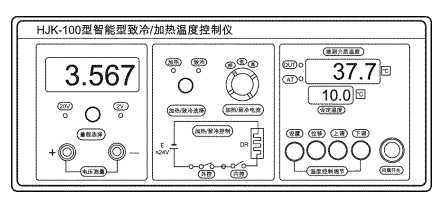
\includegraphics[height=5cm]{img//device_1.png}
% 		\end{minipage}
% 		}
% 		\subfloat[控温阱]{
% 		\label{fig:improved_subfig_b}
% 		\begin{minipage}{0.5\textwidth}
% 			\centering
% 			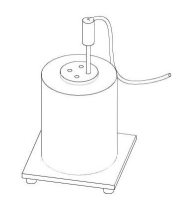
\includegraphics[height=5cm]{img//device_2.png}
% 		\end{minipage}
% 		}
% 		\caption{温度控制设备}
% 	\end{figure*}

% \section{实验结果与讨论}

% 	\subsection{数字电压读数与温度的对应关系}
% 	将测控电路接入加热阱,记录温度传感器温度为$30^{\circ}C到80^{\circ}C$对应的数字电压表示数。分别记录温度上升时和温度下降时的电压值,取平均以降低误差,如表\ref{tab:addlabel}所示。

% %%% 4 不跨栏表格
% 	%所有表格都可以通过Excel2LaTex加载项,在excel中转换成以下一串代码。需要琢磨的是调节一些细节的方法。

% 	% Table generated by Excel2LaTeX from sheet 'Sheet1'
% 	\begin{table}[H]
% 	  \centering
% 	    \begin{tabular}{cccc}
% 	    \toprule
% 	    t/$^{\circ}$C & 上升/mV & 下降/mV & 平均$V_0/mV$ \\
% 	    \midrule
% 	    30    & 271   & 280   & 275.5 \\
% 	    32.9  & 299   & 313   & 306 \\
% 	    37.8  & 336   & 363   & 349.5 \\
% 	    40.9  & 364   & 396   & 380 \\
% 	    42.7  & 387   & 414   & 400.5 \\
% 	    45    & 414   & 438   & 426 \\
% 	    50    & 460   & 489   & 474.5 \\
% 	    53    & 475   & 518   & 496.5 \\
% 	    55    & 494   & 538   & 516 \\
% 	    58    & 522   & 568   & 545 \\
% 	    60    & 540   & 588   & 564 \\
% 	    63    & 569   & 617   & 593 \\
% 	    65    & 589   & 636   & 612.5 \\
% 	    70    & 639   & 684   & 661.5 \\
% 	    73    & 669   & 711   & 690 \\
% 	    75    & 690   & 729   & 709.5 \\
% 	    78    & 721   & 753   & 737 \\
% 	    80    & 748   & 768   & 758 \\
% 	    \bottomrule
% 	    \end{tabular}%
% 	  \caption{数据记录}
% 	  \label{tab:addlabel}%
% 	\end{table}%

% %%% 5 跨栏表格
% 	%手动在table右边加上*即可

% 	% Table generated by Excel2LaTeX from sheet '打印'
% 	\begin{table*}[H]
% 	  \centering

% 	    \begin{tabular}{c|ccccc}
% 	    \toprule
% 	    \multicolumn{1}{c}{} & 油滴序号  & Q/C   & Q/e   & n     & e/C \\
% 	    \midrule
% 	    \multicolumn{1}{c}{\multirow{5}[2]{*}{静态法}} & 1     & 1.713E-19 & 1.069  & 1     & 1.713E-19 \\
% 	    \multicolumn{1}{c}{} & 2     & 5.681E-19 & 3.546  & 4     & 1.420E-19 \\
% 	    \multicolumn{1}{c}{} & 3     & 5.710E-19 & 3.564  & 4     & 1.428E-19 \\
% 	    \multicolumn{1}{c}{} & 4     & 1.292E-18 & 8.062  & 8     & 1.615E-19 \\
% 	    \multicolumn{1}{c}{} & 5     & 9.490E-19 & 5.923  & 6     & 1.582E-19 \\
% 	    \midrule
% 	    \multicolumn{1}{c}{} &       & 平均值:  & 1.551E-19 & 相对误差: & 3.169\% \\
% 	    \midrule
% 	    \multicolumn{1}{c}{\multirow{5}[2]{*}{动态法}} & 6     & 1.253E-18 & 7.821  & 8     & 1.566E-19 \\
% 	    \multicolumn{1}{c}{} & 7     & 3.174E-19 & 1.981  & 2     & 1.587E-19 \\
% 	    \multicolumn{1}{c}{} & 8     & 1.234E-18 & 7.701  & 8     & 1.542E-19 \\
% 	    \multicolumn{1}{c}{} & 9     & 9.402E-19 & 5.868  & 6     & 1.567E-19 \\
% 	    \multicolumn{1}{c}{} & 10    & 6.309E-19 & 3.938  & 4     & 1.577E-19 \\
% 	    \midrule
% 	    \multicolumn{1}{c}{} &       & 平均值:  & 1.568E-19 & 相对误差: & 2.133\% \\
% 	    \multicolumn{2}{c}{整体情况} & 平均值:  & 1.560E-19 & 相对误差: & 2.651\% \\
% 	    \bottomrule
% 	    \end{tabular}%
% 	 \caption{数据处理}
% 	\end{table*}%


% %%end--------------------插入图表------------------------%%


% %%begin------------------插入公式------------------------%%

% \section{结论}
% 美国物理学家密立根(Robert a. Millikan)在$1909 \sim 1917$年期间所做的测量微小油滴上所带电荷的工作,即油滴实验,是物理学发展史上一个具有重要意义的实验。这一实验的设计思想简明巧妙、原理清楚、设备简单、结果准确。本实验通过重做密立根的油滴实验,通过“倒过来验证”的方法从实验上验证了电荷分布的不连续性。采用的仪器是专用的密立根油滴实验仪,操作更加方便和清晰。

% 	1 需要标号、单个公式
% 		%一般来说都需要标号
% 		\begin{equation}
% 		\eta^{\prime}=\eta /[1+b /(p a)]
% 		\end{equation}

% 	2 需要标号、多个公式、不需要对齐
% 		\begin{gather}
% 		f_r=6\pi a \eta v_g   \\
% 		m=4 \pi a^{3} \rho / 3
% 		\end{gather}

% 	3 需要标号、多个公式、需要对齐
% 		\begin{align}
% 		a &= b+c+d \\
% 		x &= y+z
% 		\end{align}

% 	4 不需要标号,单个公式
% 		\[e=(1.60217733 \pm 0.00000049) \times 10^{-19} \mathrm{C}\]
% 		另一种方法:
% 		\begin{equation*}
% 		e=(1.60217733 \pm 0.00000049) \times 10^{-19} \mathrm{C}
% 		\end{equation*}

% 	5 不需要标号,多个公式,不需要对齐/需要对齐
% 		%使用对应的*版本
% 		\begin{gather*}
% 		f_r=6\pi a \eta v_g   \\
% 		m=4 \pi a^{3} \rho / 3
% 		\end{gather*}
% 		另一种方法:
% 		\begin{align*}
% 		a &= b+c+d \\
% 		x &= y+z
% 		\end{align*}

% 	6 长公式,换行,不对齐
% 		%不标号的话加上*
% 		\begin{multline}
% 		x = a+b+c+{} \\
% 		d+e+f+g
% 		\end{multline}

% 	7 长公式,换行,对齐
% 		%aligned:次环境
% 		\[\begin{aligned}
% 		x ={}&a+b+c+{} \\
% 		&d+e+f+g
% 		\end{aligned}\]

% 	8 带有左边大括号的公式
% 	\[\left\{
% 		\begin{aligned}
% 		&C_{1} \cdot \frac{d U_{C_{1}}}{d t}=\frac{1}{R_{1}} \cdot(u_{C_{2}}-u_{C_{1}})-f(u_{R_{N}}) \\
% 		&C_{2} \cdot \frac{d U_{C_{2}}}{d t}=i_{L}-\frac{1}{R_{1}} \cdot(u_{C_{2}}-u_{C_{1}}) \\
% 		&L \cdot \frac{d i_{L}}{d t}=-U_{C_{2}}
% 		\end{aligned}
% 	   \right.
% 	\]

%%end--------------------插入公式------------------------%%

\end{document}
